%
%%% Work Area I: Modeling of Fake Backgrounds %%%
%%% ----------------------------------------- %%%
%
%\chapter{Modeling of Fake Backgrounds}
%\label{chap:a-study-in-fake}
%
%%% Work Area I -> Introduction %%%
%%% --------------------------- %%%
%
\subsection{Introduction}
\label{sec:introduction}
%
Measurements of rare decays with leptons in the final state (and in general, almost all measurements with leptons) are often particularly sensitive the fake-lepton backgrounds (referred to simply as fake backgrounds from now on). %
For example, the measurement of the $B_d \rightarrow \mu \mu $ branching ratio is expected to be highly sensitive to the estimation of fake muon background due to the extremely low branching ratio ($\sim \mathcal{O}(10^{-10})$) for the decay. %
The LHCb measurement of the branching ratio of this decay measured a fake background peak of nearly equal height as the $B_d \rightarrow \mu \mu $ signal peak in the vicinity of the signal peak \cite{LHCb:2021vsc}. %
Another recent example of the sensitivity of the measurements of rare decays to the estimation of fake backgrounds is that the source of tension with the SM in the pre-2022 LHCb measurements of $R(K)$ and $R(K^{\ast})$ has been attributed to the missing estimation of the background arising from hadrons faking electrons \cite{LHCb:2017avl, LHCb:2021trn, LHCbDec2022}. % 
Also in the \mbox{ATLAS} measurements of $R(K^\ast)$, the fake backgrounds are expected to arise from the misidentification of final-state hadrons (mostly pions, kaons, and protons) as electrons or muons; as well as, to a lesser extent, from the misidentification of final-state photons as electrons via the conversion of the photon into an $e^+e^-$ pair in the detector material. %
\\\\
While it is hard to model the non-peaking partially reconstructed and combinatorial backgrounds using MC, the real peaking backgrounds can be modeled relatively well with MC. %
The remaining source of potentially peaking backgrounds, i.e., the fake backgrounds, remains hard to model in MC. %
Unlike the partially reconstructed and combinatorial backgrounds where a very large swath of processes contribute to the composition of the background and it becomes unruly to model them all, the difficulty in modeling fake backgrounds with MC simulation arises from the difficulty to accurately model the interaction of hadrons with the calorimeters (including the details of shower development) in MC simulation. %
The mechanism by which hadrons leave signatures in the detector that resemble those of leptons primarily depends on their behavior in the calorimeter. For hadrons faking electrons, this involves whether they are fully or almost fully absorbed by the EM calorimeter. For hadrons faking muons, it depends on whether they can escape the hadronic calorimeter and leave a signature in the muon spectrometer. Because MC simulations have limitations in accurately modeling these hadron–calorimeter interactions, the analysis of fake backgrounds needs to be at least partially data-driven \cite{ATLAS:2022swp}. %
It should also be mentioned that in addition to the limitations of accurate modeling, due to the low probability that a hadron fakes a lepton (usually $\sim \mathcal{O}(10^{-3})$), it also becomes computationally expensive to simulate enough events to obtain a good estimate of the fake backgrounds in MC simulation. %
%
%%% Work Area I -> Outline of the Strategy %%%
%%% -------------------------------------- %%%
%
\subsection{Outline of the Strategy}
\label{sec:outline-of-strategy}
%
Broadly speaking, conceptually, such a data-driven method has two parts: 
\begin{itemize}
    \item \textbf{Estimation of the Faking Probabilities}: Estimating, from data, the probability that a hadron fakes a lepton. %
    \item \textbf{Estimation of the Fake Background}: Transforming the faking probabilities into an estimate of the background in the signal region of the analysis. %
\end{itemize}
In this section, we outline the strategy for each of the two parts. 
\subsubsection{Estimation of the Faking Probabilities}
\label{subsec:estimation-of-faking-probabilities}
The estimation of the faking probabilities of a hadron proceeds via identifying a ``control region'' where we expect the hadrons to be the dominant source of reconstructed leptons. %
In most of the ``traditional'' analyses in ATLAS, such a control region can be obtained via inverting lepton identification criteria. %
However, there are various reasons as to why such an approach is not directly amenable to $B$-physics analyses, and especially to the electron channel of the $R(K^\ast)$ analysis:
\begin{itemize}
    \item The “traditional” analyses typically target isolated, prompt leptons. Here, ``prompt'' means that they do not originate from decays-in-flight, i.e., from heavy-flavor decays; ``isolated'' means that there is not much hadronic activity around the lepton in the calorimeter and/or in the tracker. The variables used to discriminate between a region dominated by real leptons and fake leptons rely on the assumption of high$-p_{\text{T} }$ prompt leptons, e.g., inverting the cut on the lepton identification measure or inverting the isolation variables. %
    However, since the signal leptons in $B$-physics analyses come from $B$-decays, they are not very isolated as they lie in the vicinity of the decay products of the primary vertex in which the $B$-meson originated. %
    \item The analysis working point for the electron identification in the $R(K^\ast)$ analysis is already the loosest electron identification working point that has been defined for electron reconstruction in ATLAS\footnote{In fact, this working point was developed specifically for the $R(K^\ast)$ analysis by removing the requirements on the impact parameter of the electron track from the previously loosest electron identification working point.}. % 
    %\DM{No public record of the new working point introduced, no?} %
    Thus, inverting this criterion is not possible - at least without putting in considerable efforts into creating an even looser working point.
    \item Even if a variable, whose selection can be inverted to differentiate between signal leptons and fake leptons, can be found, extracting a fake-enrinched region via subtracting the non-fake backgrounds is much less straightforward compared to the “traditional” analyses where the real background component is usually defined by a small set of well modeled processes (typically top and electroweak processes). %
    In particular, the fake-lepton contributions in this control region, just like the signal in the signal region, will be swamped by combinatorial as well as partially reconstructed decays. 
\end{itemize}
We thus need to develop a different approach to obtain a fake-enriched region. %
We adopt and expand the approach wherein we utilize the decays of $B$-hadrons to unambiguously identify hadrons and thus isolate a hadron-enriched region that we then use to derive the faking probabilities of the said hadron. %
To estimate the probability that a hadron $h$ fakes a lepton $\ell$, i.e., $P(h\to\ell)$, we first identify a decay channel of a heavier hadron that can be used to tag the hadron of interest. %
%\begin{itemize}
%    \item The decay channel has the hadron of interest, i.e., $h$ as a final state.
%    \item We can trigger the event using the final states of the decay. Since ATLAS can only trigger on leptons and not hadrons\footnote%{ATLAS can also trigger on photons and jets. However, among the hadrons and the leptons, it can only trigger on leptons.}, this means %the decay channel should have at least one lepton.
%    \item We can ``easily'' isolate the decay channel in data in the presence of background, i.e., it forms an unambiguous peak in some %discriminating variable. Though not strictly, it practically implies the following properties:
%    \begin{itemize}
%        \item The $\sigma \times {\mathrm{BR}}$ of the decay channel is relatively high.
%        \item We are able to fully reconstruct the decay so that it forms an unambiguous peak in the reconstructed mass of the %parent hadron.
%    \end{itemize}
%\end{itemize}
A natural choice for the parent hadron is a $B$-hadron since it automatically puts us in a phase-space that is not dissimilar to the phase-space that would be occupied by hadrons faking leptons in our analysis. 
%For example, if we instead use a $\Lambda_b^0$ decay channel, the fact that it's much longer lived than the $B$-hadron would make the hadrons produced via its decay too displaced. 
In particular, we select $B^+\to J/\psi(\to \mu^+\mu^-)K^+$ to tag the $K^\pm$s and $B^0\to J/\psi(\to \mu^+\mu^-) K^{\ast 0}(\to K^+\pi^-)$ to tag the $\pi^\pm$s.
%    \begin{itemize}
        %\item 
While ATLAS cannot effectively discriminate between the $K^\pm$ and $\pi^\pm$, the fact that they come from a common $K^{\ast 0}$-vertex provides us with a good enough handle on their particle identification -- based on checking if assigning the $K^+$ mass hypothesis to the positively charged meson (and $\pi^-$ mass hypothesis to the negatively charged meson) leads to a dimeson mass that is closer to the PDG value of the $K^{\ast 0}$ mass compared to reverting the mass-hypothesis assignments. This strategy has an identification accuracy of $\sim 85\%$. %
Furthermore, our trained GNNs can discriminate between $K^\pm$s and $\pi^\pm$s (albeit in this specific topology) with a $>95\%$ accuracy. Hence, we can tag the $\pi^\pm$s with high enough accuracy.
%    \end{itemize}
%\end{itemize}
%Notice that using the muon channel decay for the $J/\psi$ is much more favorable than using the electron channel decay of the same resonance due to the ATLAS trigger design. %
\\\\
Once we have tagged the hadrons, in essence, we can simply count the number of those hadrons that are also reconstructed as leptons via matching the Inner Detector (ID) tracks of the hadrons to the lepton tracks. %
We derive the following faking probabilities using this approach: 
\begin{itemize}
    \item $P(K^\pm \to e^\pm)$
    \item $P(\pi^\pm \to e^\pm)$
    \item $P(K^\pm \to \mu^\pm)$
    \item $P(\pi^\pm \to \mu^\pm)$
\end{itemize}
where, in this context, $\to\equiv \xrightarrow[\text{reconstructed as}]{}$ and \underline{not} a decay (albeit some of the misidentifications come from in-flight decays). The $K^\pm\to \mu^\pm$ probabilities had previously been derived in ATLAS, however, they were not parametrized in a way to be useful. We fix the parametrization (by parametrizing them in the $2$D space of $p_{T}$ and $\eta$ of the hadron), and the rest of the probabilities are derived for the first time.  %%
%
%
\subsubsection{Estimation of the Fake Background}
Once we have the faking probabilities of the hadrons, the strategy to estimate the fake background in the signal region is to utilize MC samples of all possible background processes that none or one lepton in the final state and can reasonably contribute to a peaking fake background. %
However, it is important to note that we do not rely on the MC modeling of the process through which a hadron fakes a lepton, rather, we will utilize the faking probabilities that we derived in the previous section by selecting the relevant hadrons in the MC sample and assigning them with the relevant probability to fake a lepton. %
In using the MC samples of the fake background processes, what we are utilizing from the MC simulation is the decay kinematics. %
The strategy to estimate the fake background along these lines is as follows:
\begin{itemize}
    \item Prepare an ensemble of MC samples of all decays that can `reasonably' contribute to a fake background that peaks in the signal region. This is discussed in detail in \ref{subsec:preparation-of-the-mc-samples}. Notice that there are many fake leptons contributions from a huge swath of processes, but we are concentrating on those which are (potentially) peaking in the signal region since the others are contributing to the continuum, which is modeled from a fit to the data in sidebands. %
    \item Perform the entire analysis on these MC samples, but without requiring any selection cuts that are specific to lepton identification, that is, offline lepton identification cuts as well as online, i.e., trigger-level, lepton identification cuts. This is discussed in detail in \ref{subsec:performing-analysis-w-o-lepton-identification-cuts}.
    \item Correct for the removal of the offline lepton identification cuts by weighing each event by a faking probability that is calculated using the previously derived faking probabilities of the hadrons. This is discussed in detail in \ref{subsec:applying-the-faking-probabilities}. %
    \item Correct the kinematic differences between hadron track reconstruction 
    and lepton track reconstruction. This is discussed in detail in \ref{subsec:kinematic-corrections}. %
    \item Correct for the removal of the online lepton identification cuts by weighing each event using appropriate ``trigger weights''. This is discussed in detail in \ref{subsec:applying-trigger-weights}. %
\end{itemize}
A schematic diagram of this strategy is shown in \ref{fig:fake-rate-transfer-strategy}. %
\begin{figure}[!ht]
    \centering
    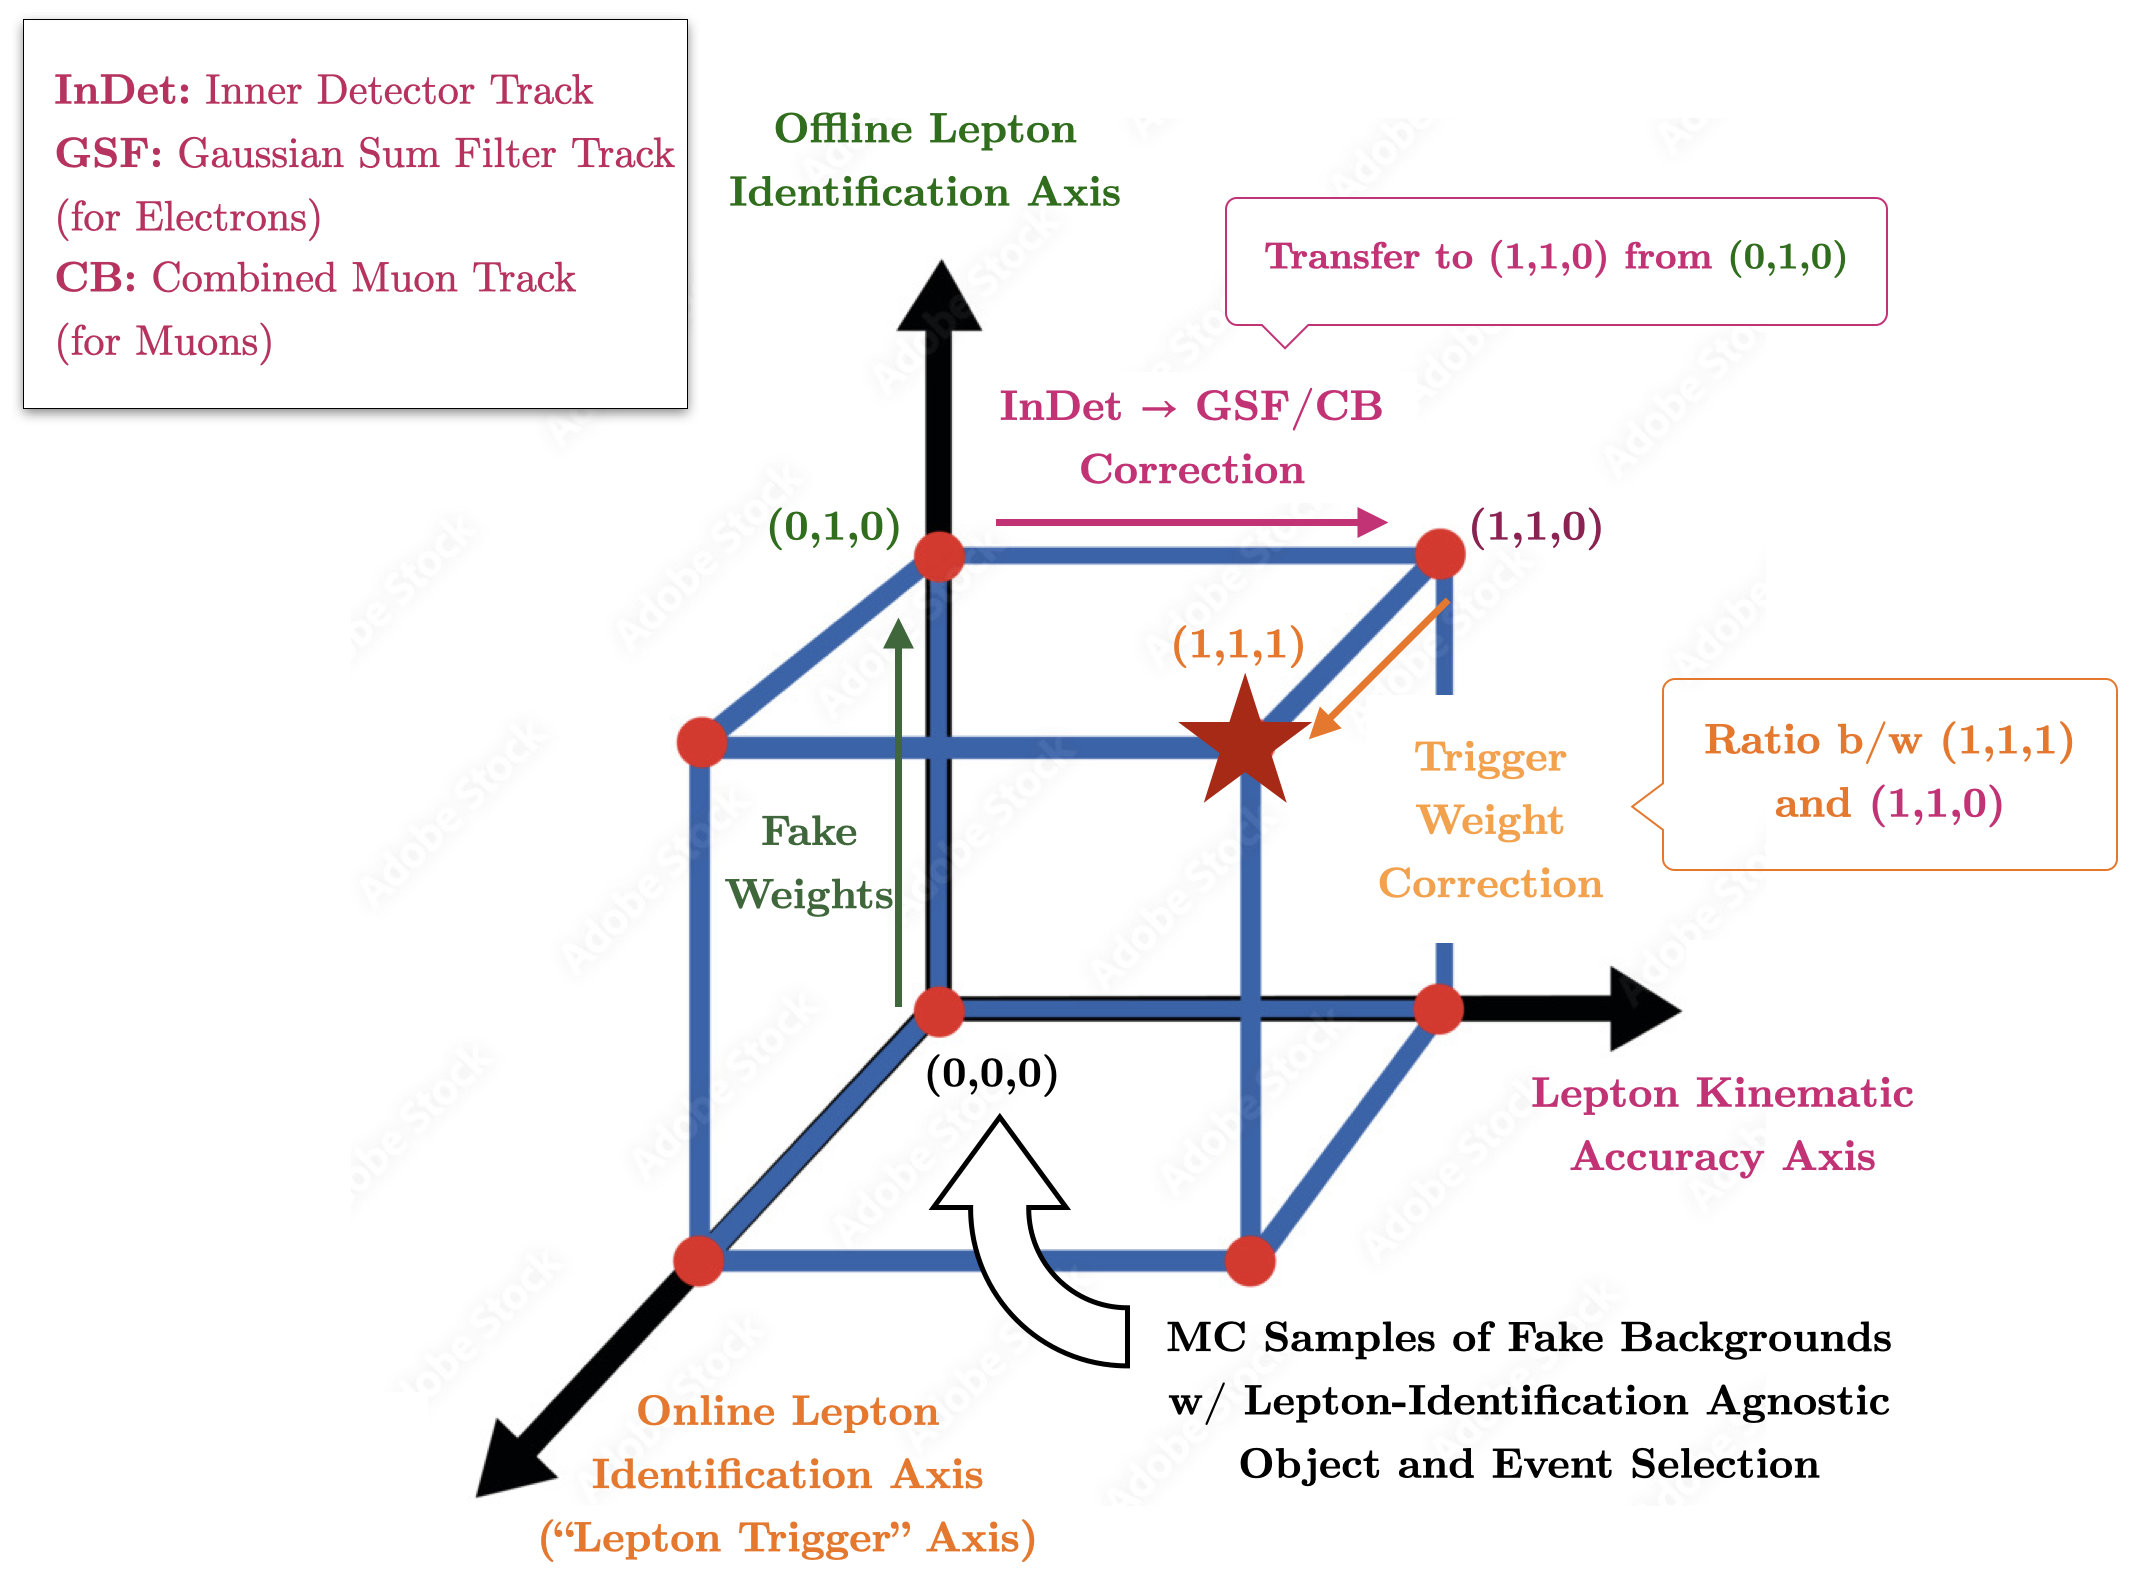
\includegraphics[width=0.95\textwidth]{figures/FakesEstimation/FakeRateTransferStrategy.png}
    \caption{Schematic diagram of the strategy to estimate the fake background in the signal region. The faking probabilities are derived using a hadron-enriched region and then applied to the MC samples of all decays that can reasonably contribute to the fake background. The faking probabilities are then corrected for the removal of lepton identification cuts and kinematic differences.}
\end{figure}
\label{fig:fake-rate-transfer-strategy}
Notice that while this approach, as formulated above, is general, the details of the implementation are specific to the analysis at hand. Particularly due to two main reasons:
\begin{itemize}
    \item The ensemble of MC samples of all decays that can `reasonably' contribute to the fake background depends on the signal signature of a specific analysis. For example, $B^0\to D^-(\to K^+\pi^-\pi^-)\pi^+$ can fake a $B_d \rightarrow K^{\ast } ee$ signal if two of the three pions are misidentified as electrons. However, even if two of the four mesons are misidentified as muons, it is highly unlikely to fake a $B \rightarrow \mu \mu $ signal since the reconstructed mass of such a fake $B$-meson will be significantly lower than the mass of the $B$-meson (and would thus lie outside the signal region). %
    \item As will be discussed in the following, the kinematic corrections and the corrections for the online lepton identification cuts are to be derived using a reference channel. % 
    The reference channel is chosen to be as similar to the signal channel as possible, and thus, this choice is also specific to the analysis at hand. %
\end{itemize}
\subsection{Estimation of the Faking Probabilities}
\label{sec:tag-and-fake-method}%
%
\subsubsection{Estimation of $P(K^\pm\to\ell^\pm)$}
\label{subsec:estimation-of-K-to-ell}
The faking probabilities of the kaons are derived using the decay channel $B^\pm\to J/\psi(\to \mu^+\mu^-)K^\pm$. %
In particular, the $B^\pm\to J/\psi(\to \mu^+\mu^-)K^\pm$ candidates are reconstructed by fitting two well-identified muon tracks and an additional charged track to a common vertex. %
No particle identification criteria are applied to the additional charged track. %
Simple cuts on the quality of the $B$-vertex fit, the displacement of the $B$-vertex from the primary vertex, and the pointing angle are applied to suppress the combinatorial background. %
Finally, the reconstructed mass of the $B^\pm$-meson is calculated after constraining the mass of the dimuon system to the PDG value of the $J/\psi$ mass. %
Now, two yields are extracted:
\begin{itemize}
    \item The yield of all of the $B^\pm$-candidates is obtained using an unbinned extended maximum likelihood fit to the reconstructed mass of the $B^\pm$-candidates. %
    This yield is our roundabout way of obtaining the number of kaons, i.e., $N_{K^\pm}$. Recall that we are not really interested in the $B^\pm$-decay itself, but rather, we simply use this decay to tag the kaons. An example mass fit to the reconstructed $B$-mass to extract the yield of $N_{K^\pm}$ is shown in \ref{fig:fakeMuonMassFitForKaons}. %
    \item We select a subset of the $B^+$-candidates wherein we can match the ID track of the kaon to the ID track of a reconstructed lepton (at a given lepton identification working point). The yield of all such $B^+$-candidates is now obtained using an unbinned extended maximum likelihood fit to the reconstructed mass of the $B^+$-candidates. %
    This yield is our roundabout way of obtaining the number of kaons that fake a lepton, i.e., $N_{K^\pm\to\ell^\pm}$. %
    An example mass fit to the reconstructed $B$-mass to extract the yield of $N_{K^\pm\to\ell^\pm}$ is shown in \ref{fig:fakeMuonMassFitForKaons}. %
\end{itemize}
\begin{figure}[!ht]
    \centering 
    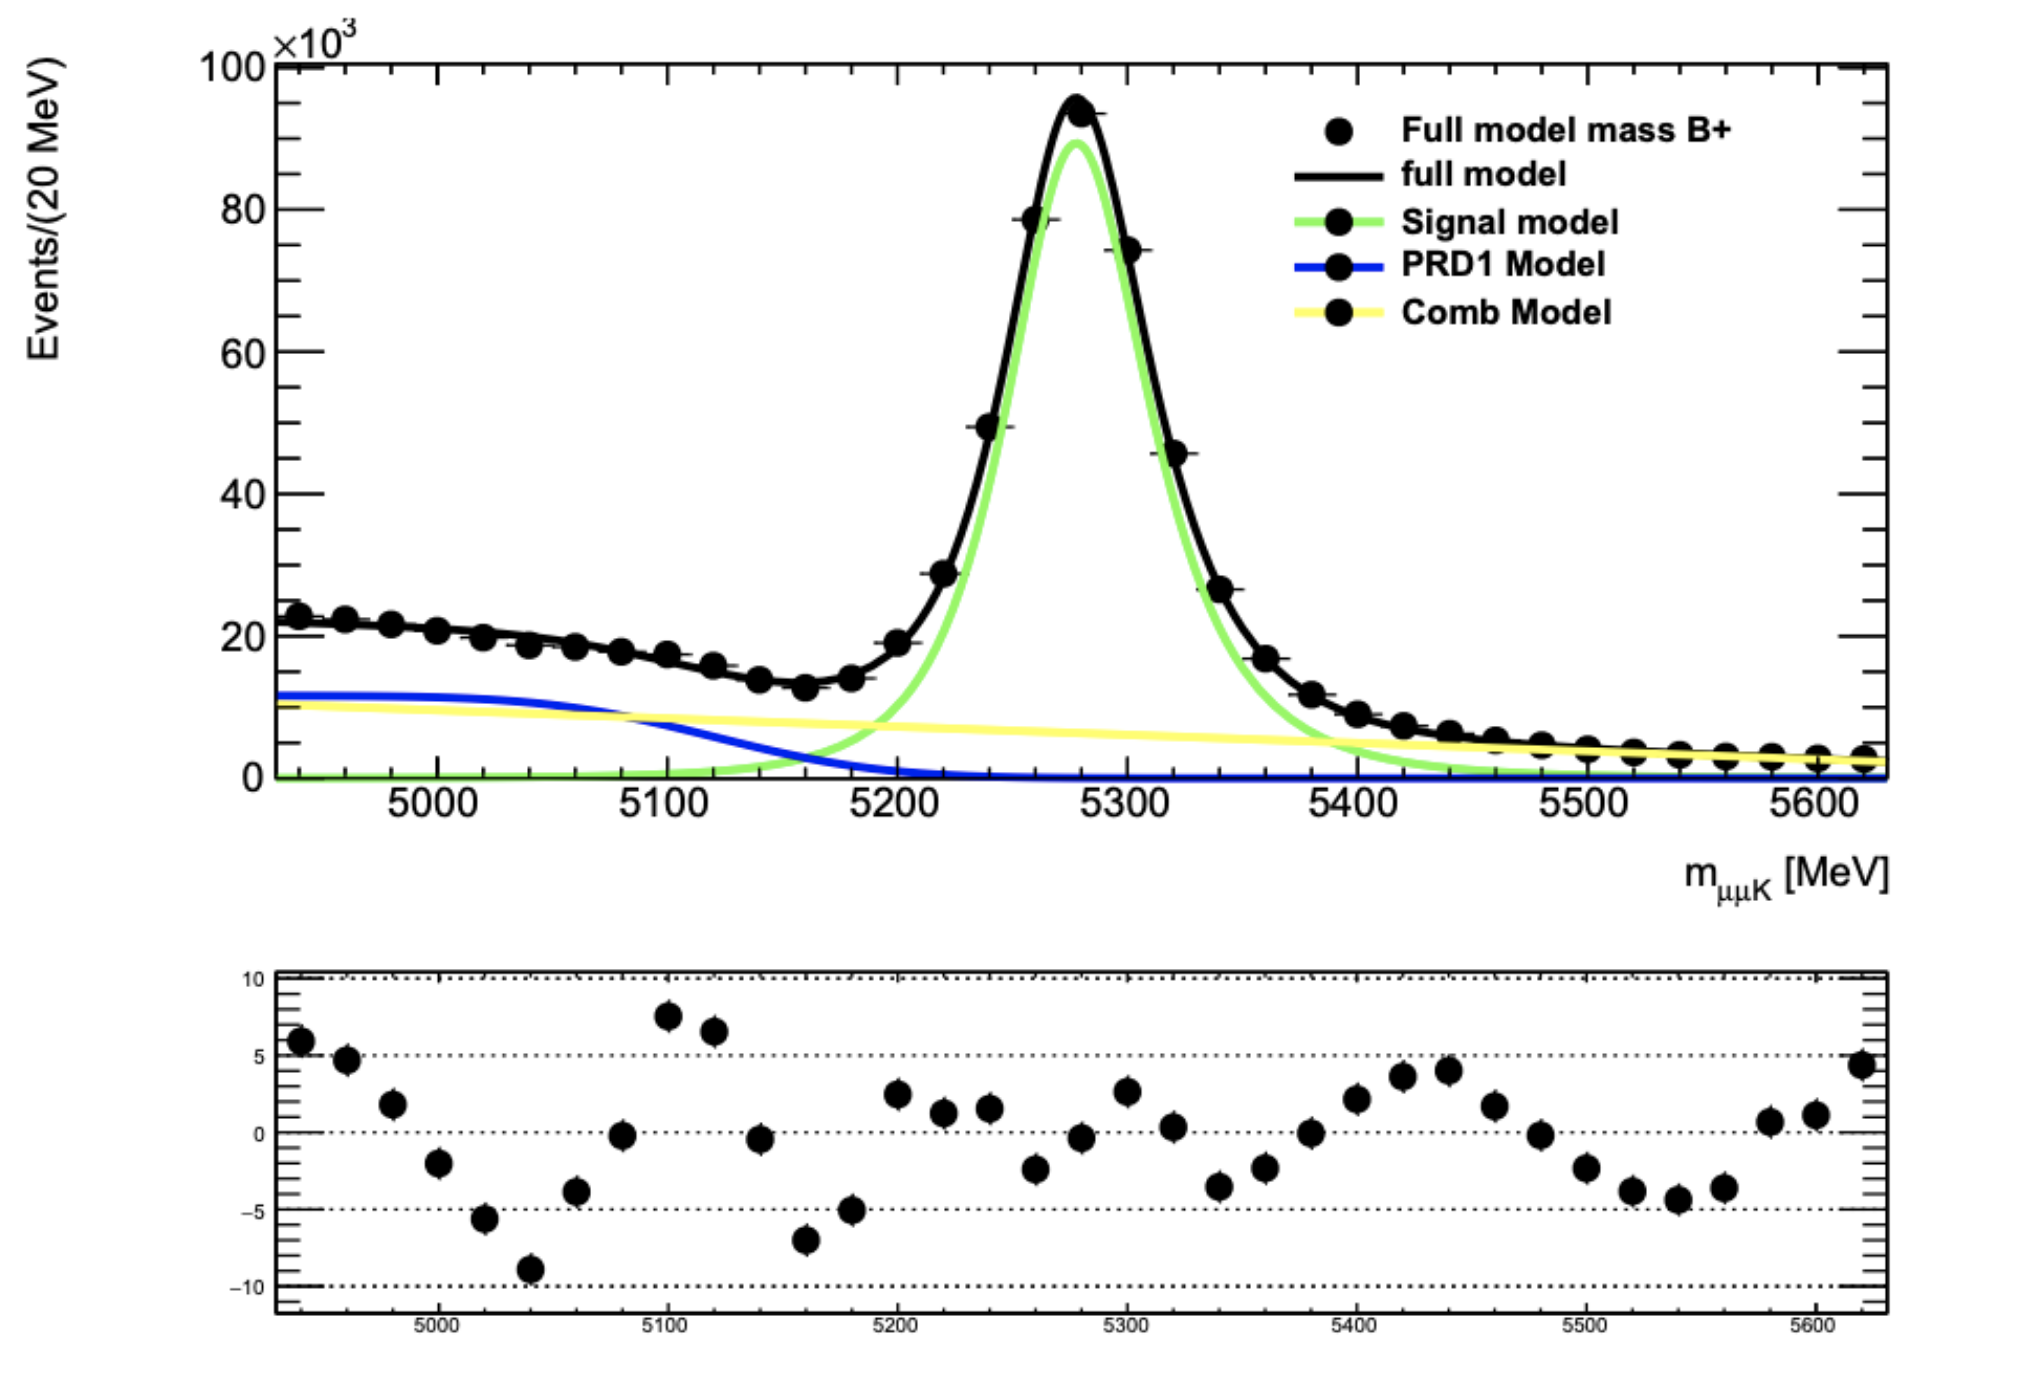
\includegraphics[width=0.45\textwidth]{figures/FakesEstimation/fakeMuonFitDenom.png}
    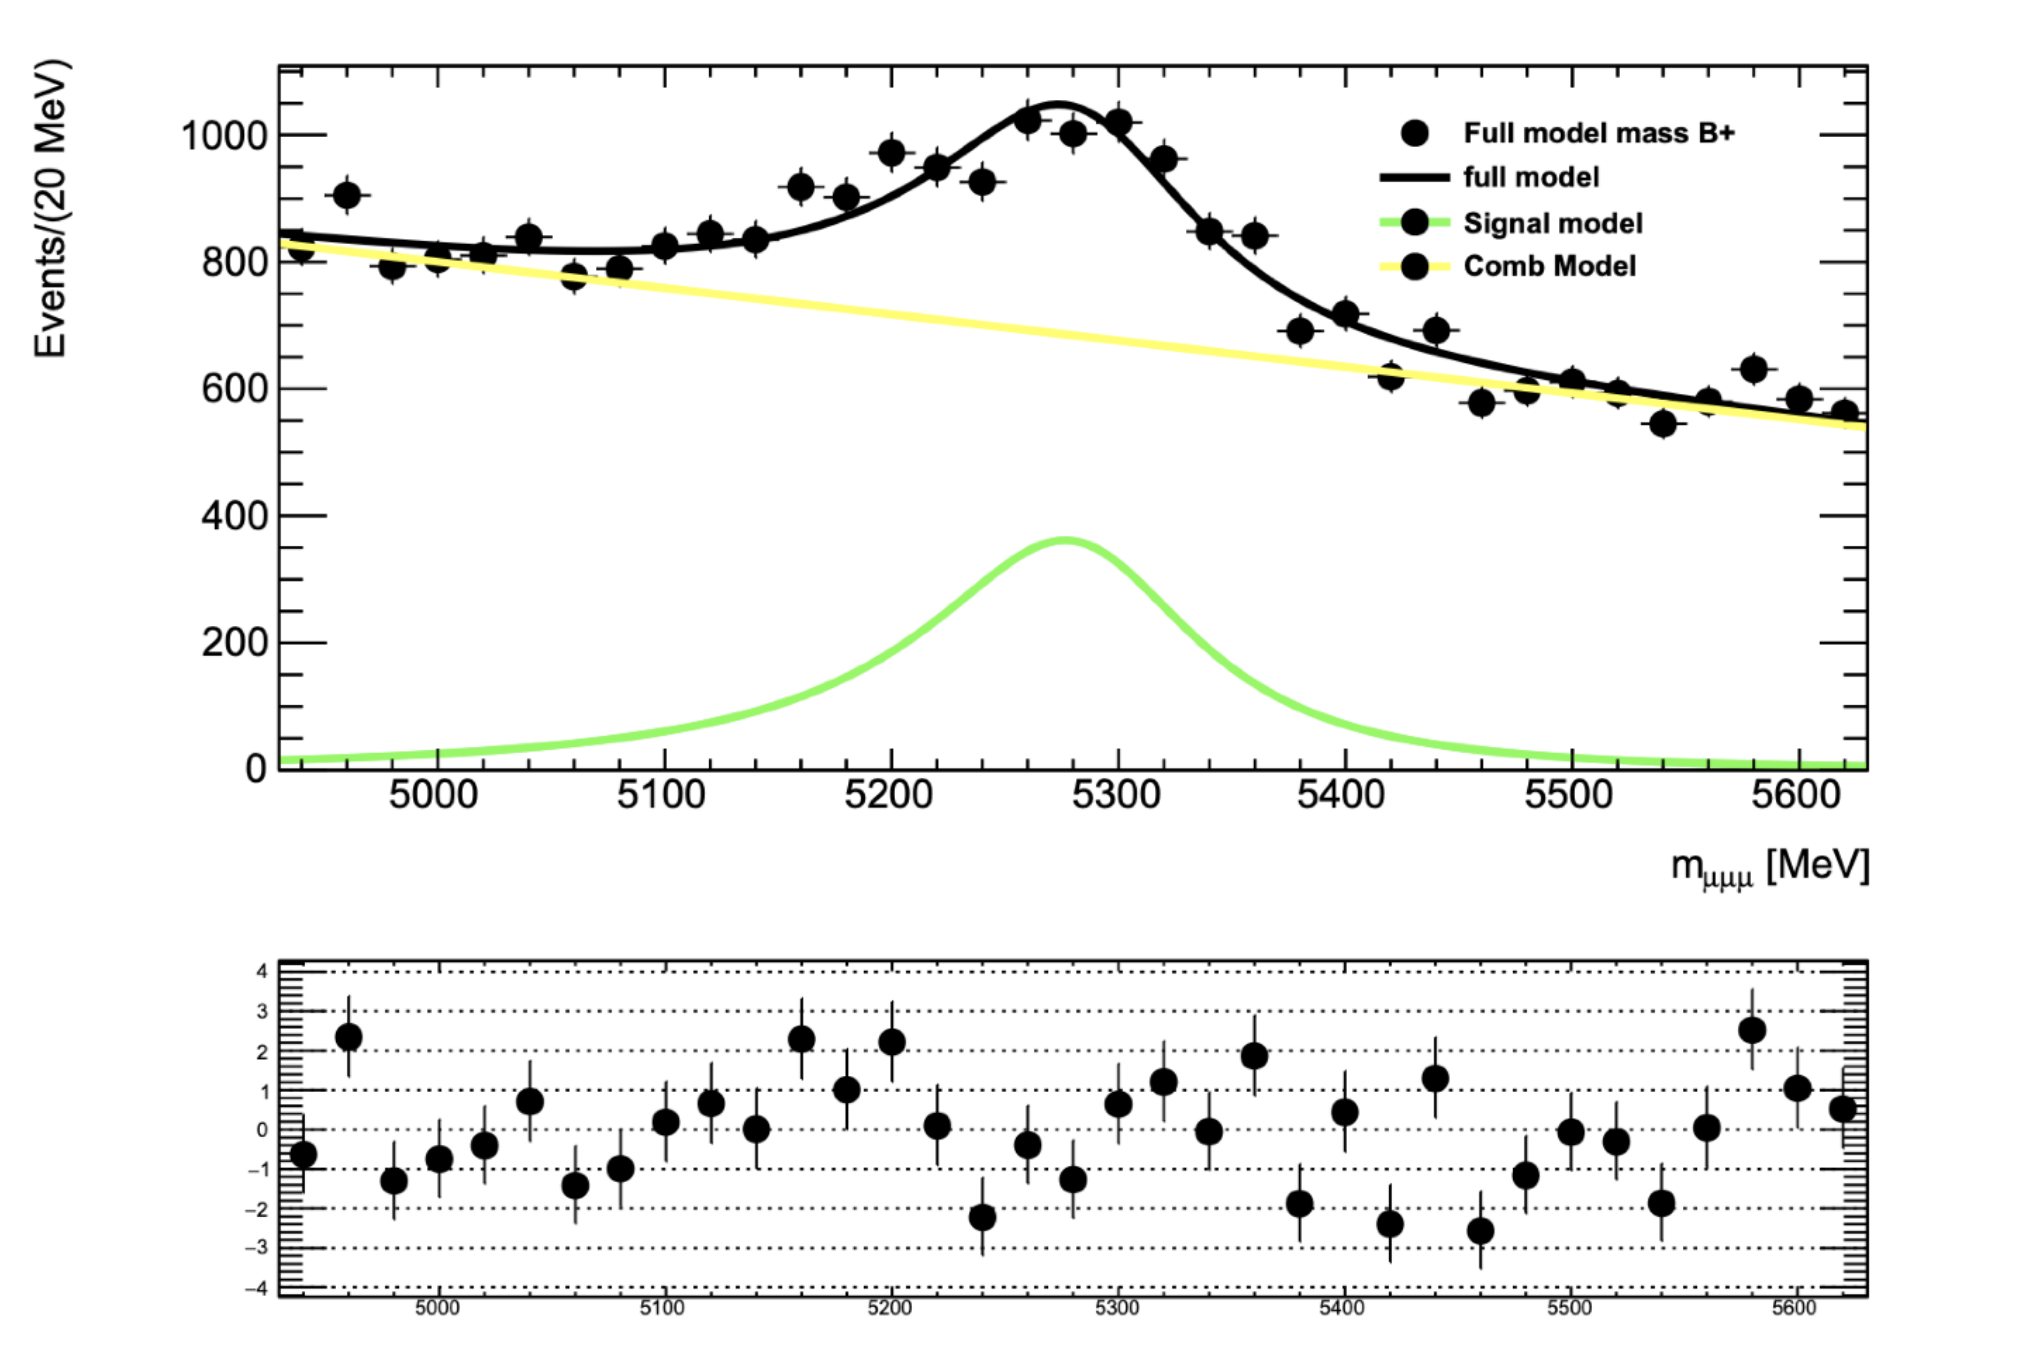
\includegraphics[width=0.45\textwidth]{figures/FakesEstimation/fakeMuonFitNumer.png}
    \caption{Example mass fit to the reconstructed $B$-mass to extract the yield of $N_{K^\pm}$ (left) and $N_{K^\pm\to\ell^\pm}$ (right).}
    \label{fig:fakeMuonMassFitForKaons}
\end{figure}
Finally, the faking probability of the kaons is obtained as:
\begin{equation}
    P(K^\pm\to\ell^\pm) = \frac{N_{K^\pm\to\ell^\pm}}{N_{K^\pm}}
\end{equation}
This procedure is repeated in bins of $p_{\text{T}}$ of the kaon ID track for both the Barrel and the Endcap regions of the ATLAS detector. %
The results for the faking probabilities of the kaons are shown in \ref{fig:K-to-ell-faking-probabilities}. %
\begin{figure}[!ht]
    \centering 
    \includegraphics[page=2,width=0.45\textwidth]{figures/FakesEstimation/compare.BJPsiK.KaonFakes.c1.pdf}
    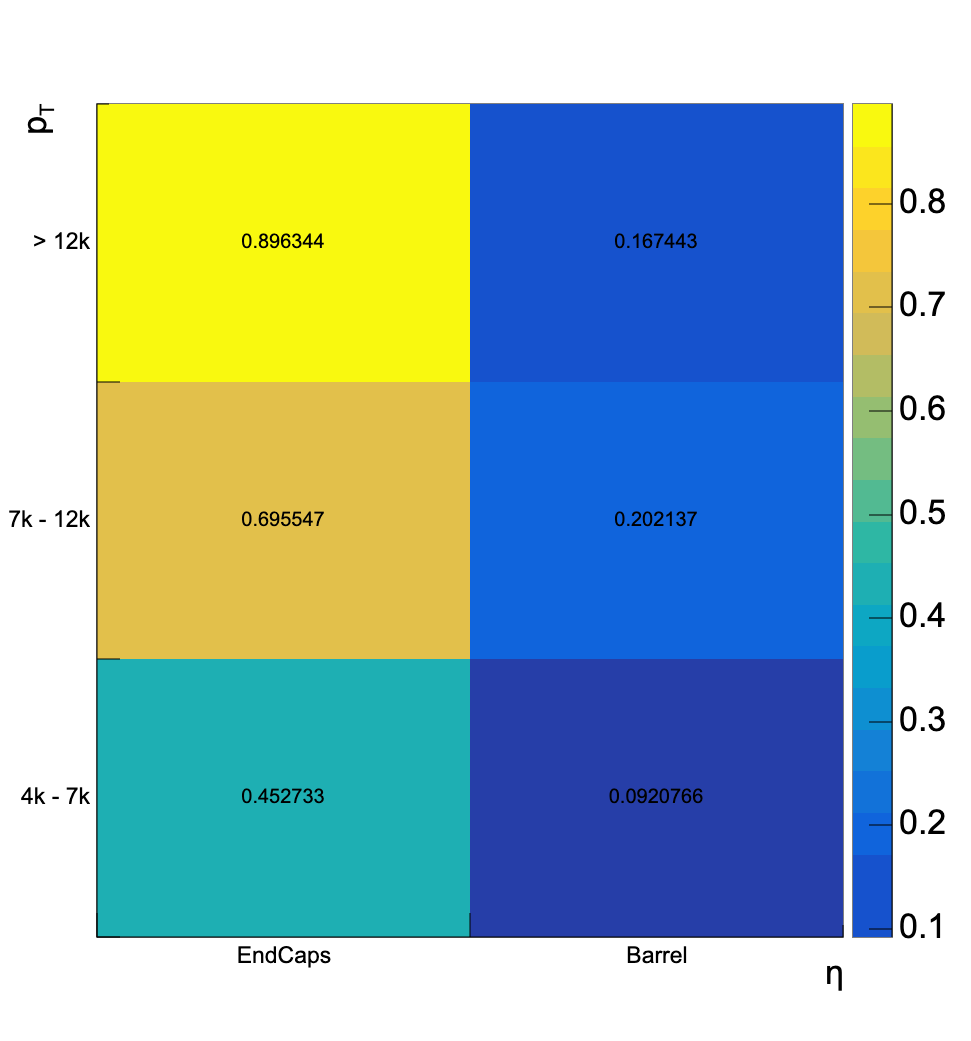
\includegraphics[width=0.45\textwidth]{figures/FakesEstimation/fakeRatesKaonsData.png}
    \caption{{\textbf{Left:}} $P(K^\pm \to e^\pm)$ in Barrel and Endcap, 
    {\textbf{Right:}} $P(K^\pm \to \mu^\pm)$ in Barrel and Endcap.}
    \label{fig:K-to-ell-faking-probabilities}
\end{figure}
\subsubsection{Estimation of $P(\pi^\pm \to \ell^\pm)$}
The faking probabilities of the pions are derived using the decay channel $B^0\to J/\psi(\to \mu^+\mu^-)K^{\ast 0}(\to K^+\pi^-)$. %
The $B^0$-candidates are reconstructed by fitting two well-identified muon tracks and two additional charged tracks to a common vertex. %
No particle identification criteria are applied to the additional charged tracks (recall that ATLAS cannot effectively distinguish between different mesons, certainly not above $1{\ {\text{GeV}}}$). %
Simple cuts on the quality of the $B$-vertex fit, the displacement of the $B$-vertex from the primary vertex, and the pointing angle are applied to suppress the combinatorial background. %
At this point, we check if assigning the $K^+$ mass hypothesis to the positively charged meson (and $\pi^-$ mass hypothesis to the negatively charged meson) leads to a dimeson mass that is closer to the PDG value of the $K^{\ast 0}$ mass compared to reverting the mass-hypothesis assignments. %
Depending on which mass hypothesis assignment leads to a dimeson mass that is closer to the PDG value of the $K^{\ast 0}$ mass, we assign the positively charged meson as either a $K^+$ or a $\pi^+$ and the negatively charged meson as either a $\pi^-$ or a $K^-$. %
This decision can also be made using our trained GNNs, which show a better discrimination accuracy than the ``closer mass’’ method, but this does not affect the rest of the reasoning, and hence, we try to keep the discussion as simple as possible. %
This assignment is then used for two different purposes:
\begin{itemize}
    \item The assigned mass hypotheses are used to calculate the reconstructed $B^0$-meson mass. %
    \item The assigned mass hypotheses are also used to isolate the $\pi^\pm$ from the $K^\mp$ in the calculation of the faking probabilities. For example, in the following, we will focus on deriving the faking probabilities of the positively charged meson, i.e., $P(\pi^+ \to \ell^+)$. The negatively charged meson is treated in a similar way. %
\end{itemize}
In order to isolate the subset of $B^0$-candidates wherein the positively charged meson track is a $\pi^+$, we simply select the subset wherein the positively charged meson track is assigned the $\pi^+$ mass hypothesis via the procedure described above. %
Finally, the reconstructed mass of the $B^{\ast 0}$-meson is calculated after constraining the mass of the dimuon system to the PDG value of the $J/\psi$ mass. %
Now, two yields are extracted:
\begin{itemize}
    \item The yield of all of the $B^0$-candidates is obtained using an unbinned extended maximum likelihood fit to the reconstructed mass of the $B^0$-candidates. %
    This yield is our roundabout way of obtaining the number of positively charged pions, i.e., $N_{\pi^+}$. Recall that we are not really interested in the $B^0$-decay itself, but rather, we simply use this decay to tag the pions.
    \item We select a subset of the $B^0$-candidates wherein we can match the ID track of the (positively charged) pion to the ID track of a (positively charged) reconstructed lepton (at a given lepton identification working point). The yield of all such $B^0$-candidates is now obtained using an unbinned extended maximum likelihood fit to the reconstructed mass of the $B^0$-candidates. %
    This yield is our roundabout way of obtaining the number of (positively charged) pions that fake a (positively charged) lepton, i.e., $N_{\pi^+\to\ell^+}$. %
\end{itemize}
Finally, after repeating the equivalent procedure for the negatively charged pions, the faking probability of the pions is obtained as:
\begin{equation}
    P(\pi^\pm\to\ell^\pm) = \frac{N_{\pi^\pm\to\ell^\pm}}{N_{\pi^\pm}}
\end{equation}
This procedure is repeated in bins of $p_{\text{T}}$ of the pion ID track for both the Barrel and the Endcap regions of the ATLAS detector. %
The results for the faking probabilities of the pions are shown in \ref{fig:pi-to-ell-faking-probabilities}. %
It should be noted that the faking probabilities that are shown here are from MC, and the equivalent probabilities are not yet derived using data (as the relevant data samples needed for performing this analysis are yet in the production stage).
\begin{figure}[!ht]
    \centering 
    \includegraphics[page=2,width=0.45\textwidth]{figures/FakesEstimation/compare.BEEKstTruth.PionFakes.c1.pdf}
    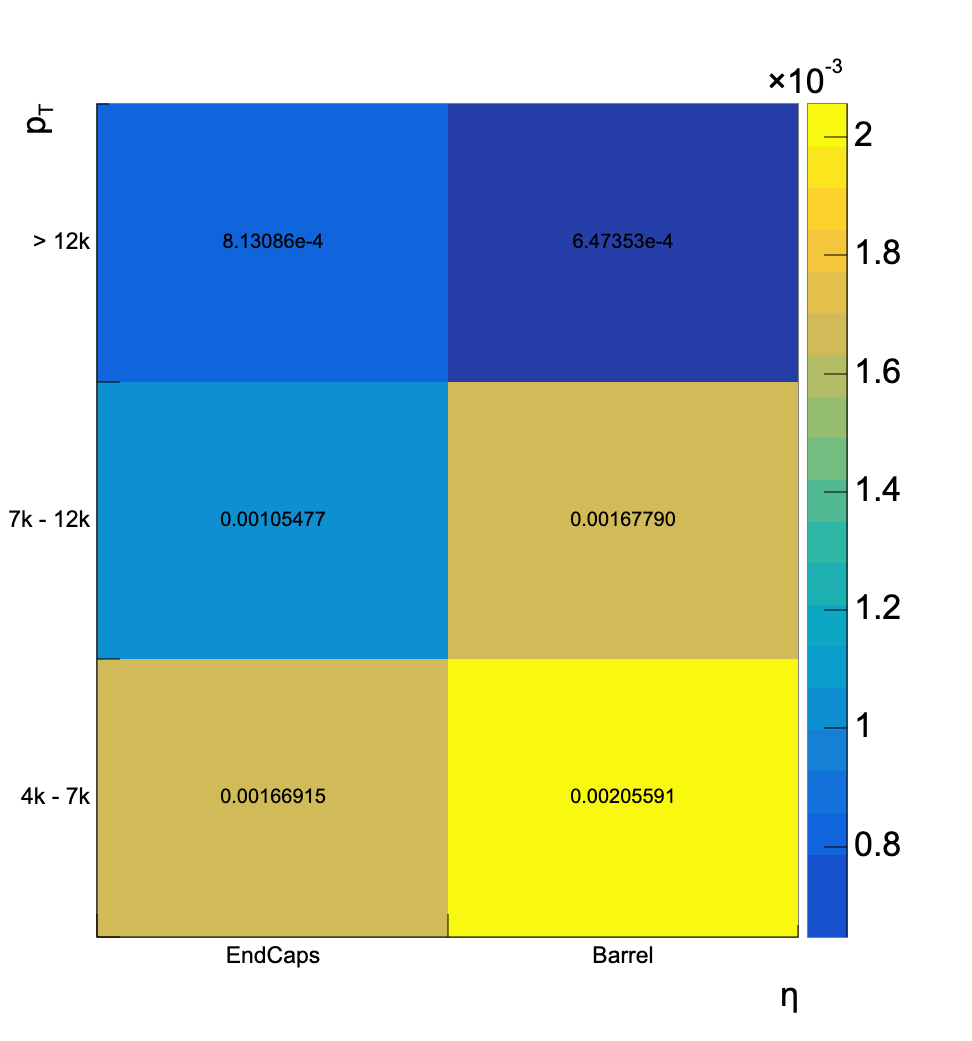
\includegraphics[width=0.45\textwidth]{figures/FakesEstimation/fakeRatesPionsMC.png}
    \caption{{\textbf{Left:}} $P(\pi^\pm \to e^\pm)$ in Barrel and Endcap, 
    {\textbf{Right:}} $P(\pi^\pm \to \mu^\pm)$ in Barrel and Endcap.}
    \label{fig:pi-to-ell-faking-probabilities}
\end{figure}
Notice that $P(\pi^\pm \to e^\pm) > P(K^\pm \to e^\pm)$, while $P(\pi^\pm \to \mu^\pm) < P(K^\pm \to \mu^\pm)$. %

\subsubsection{Systematic Bias in Evaluation of the Faking Probabilities}
Two potential sources of systematic bias in the procedure adopted to evaluate the faking probabilities are considered: bias due to vertexing and bias due to the use of a specific decay channel. %
Both of these potential biases can be broadly viewed as arising out of the concern that we use a specific decay channel to estimate the probabilities that a hadron fakes a lepton, and then we plan to use these probabilities for various other decay channels. %
We do not expect that these systematics will be large, and the statistical uncertainty in the measurement will still dominate over the systematical ones. % 
%\DM{Omitting the comment that the fake background itself is expected to be small...} %
We nevertheless comment on these two sources of uncertainty in Appendix-\ref{sec:app:fake-systematics} and show that they are indeed small. %
\subsection{Estimation of the Fake Background}
\label{sec:estimation-of-fake-background-in-signal-region}
\subsubsection{Preparation of the MC Samples}
\label{subsec:preparation-of-the-mc-samples}
We describe here the procedure followed to identify the decays that can reasonably contribute to the fake background in the signal region and potentially peak in the signal region. %
Due to the complicated FSS of the $R(K^\ast)$ analysis, we need to employ a more systematic approach to identify the decays that can reasonably contribute to the fake background. %
%\DM{Add a big comment saying that this discussion is for the $R(K^\ast)$ analysis because the signature for $B \rightarrow \mu \mu $ is simple and so we handpick the 8 decays that can fake the signal.}
In order to identify such decays, we follow a three-step process:
\begin{itemize}
    \item Identify the possible parent hadrons whose decays can contribute to the fake background.
    \item Identify the possible FSSs of the decays of the parent hadrons that can contribute to the fake background.
    \item Compile a list of all decays with the FSSs identified in the previous step for each of the parent hadrons identified in the first step.
\end{itemize}
\subsubsection*{Identification of the Parent Hadrons}
We consider hadrons with $m\in[\ 4.0,\ 6.0\ ]\ \text{GeV}$, i.e., the nominal fit-range for $m(B)$: $B^0$, $B^+$, $B_s^0$, $\Lambda_b^0$.
\subsubsection*{Identification of the FSS}
We parametrize the FSS by the number of different stable particles therein: $(n_e, n_h, n_\gamma, n_\nu)$. %
To impose certain constraints on the FSS, we consider the following reasoning: if the parent hadron decays into a final state with $k$ particles and the reconstructed $B$-candidate has $\leq k$ particles, then the reconstruction will necessarily not capture all the particles in the final state of the actual decay. % 
Such cases are referred to as ``partially reconstructed'' decays. On average, the reconstructed $B$-candidate will have a lower mass than the actual parent hadron. %
On the other hand, if the reconstructed $B$-candidate has $> k$ particles, then the reconstruction will necessarily have more particles than the actual decay, and hence, the reconstructed $B$-candidate will have a higher mass than the actual parent hadron. %
Such cases are referred to as ``overly reconstructed'' decays. %
In the case of the $R(K^\ast)$ analysis, we are interested in the FSS of $2$ leptons and $2$ hadrons. %
We thus impose the following (rather liberal) constraints on the FSS to be considered as potentially contributing to the fake background:
        		\begin{itemize}
                    \item $n_\ell < 2$. This is the defining condition for a fake background, given that our signal signature has two leptons. %
                    \item $n_\gamma + n_\nu \leq 2$. The reconstructed $B$-candidate would be too soft otherwise. We will call such a background this ``too partially reconstructed''.
	        		\item $2\leq n_e + n_h \leq 6$. The reconstructed $B-$candidate would be too soft or too hard otherwise. We will call the latter type of backgrounds ``too overly reconstructed''.
	        		\item $n_h \geq 1$. The reconstructed $B$-candidate would be too overly reconstructed otherwise. 
		        \end{itemize}
%\NTH{Huge objections to the content in the list above}. %
Purely algebraically, there are $120$ possible FSSs that satisfy the above constraints. %
In order to further narrow down this list, for any given FSS that is different than signal signature (SS), we need to understand the way in which it'd resemble the SS after reconstruction. For example, if the FSS is $hhhh$, it can be reconstructed as $hhee$ due to two $h\to e$ misidentifications. %
The more the number of such transformations that are needed to take a given FSS to the SS:
			\begin{itemize}
				\item It is less likely to be a dominant background because each transformation has a smaller than $1$ probability of happening (particularly for hadron $\to$ lepton misidentifications, the probability is $\sim 10^{-3}$).
				\item It is less likely to be peaking around the signal peak, because each transformation introduces an inaccuracy in the reconstructed mass of the $B$-meson -- resulting either in a non-peaking background, a background with a very broad peak, or a background with a peak that is shifted sufficiently away from the signal peak.
			\end{itemize}
We consider the set of transformations for taking an FSS to the SS outlined in \ref{tab:list-transformations}. %
\begin{table}[ht]
\centering
\begin{tabular}{|c|p{8cm}|c|}
\hline
\textbf{Notation} & \textbf{Transformation} & \textbf{Leads To...} \\
\hline
$\mathcal{O}_{h}^\dagger$ & An astray hadron is picked up from the environment by the reconstruction algorithm. & Overly Reconstructed Background \\
$\mathcal{O}_{\ell}^\dagger$ & An astray lepton is picked up from the environment by the reconstruction algorithm. & Overly Reconstructed Background \\
$\mathcal{O}_{h}$ & A hadron (from the signature) is missed by the reconstruction algorithm. & Partially Reconstructed Background \\
$\mathcal{O}_{\ell}$ & An electron (from the signature) is missed by the reconstruction algorithm. & Partially Reconstructed Background \\
$\mathcal{O}_{X=\gamma,\nu}$ & A photon/neutrino (from the signature) is missed/ignored by the reconstruction algorithm. & Partially Reconstructed Background \\
$\mathcal{O}_{h\to \ell}$ & A hadron (from the signature) is reconstructed as an electron. & Fake Background \\
$\mathcal{O}_{\ell\to h}$ & A lepton (from the signature) is reconstructed as a hadron. $\sim$Negligible & Fake Background \\
$\mathcal{O}_{\gamma \to ee}$ & A photon (from the signature) pair--produces an electron--positron pair in the detector material. & Fake Background \\
\hline
\end{tabular}
\caption{Summary of reconstruction transformations and their resulting background types.}
\label{tab:list-transformations}
\end{table}
%\NTH{Issues with the table!!}
For example, an FSS of $hhh$ can be transformed to the SS $hhee$ via the simple transformation $\mathcal{O}_{h\to e}\mathcal{O}^\dagger_h$. %
Thus, in addition to being a fake background, it will also be an overly reconstructed background. %
We disregard an FSS if it requires an ``unreasonable'' number of transformations to take it to the SS, resulting in the list of FSSs relevant to the $h\to\ell$ fake background outlined in \ref{tab:potential-fake-fss}. %
\begin{table}[!ht]
    \centering
    \begin{tabular}{||c|c||}
        \hline
        \textbf{FSS} & \textbf{Transformations to SS} \\
        \hline 
        $hhhhhh$ & $\mathcal{O}^2_h\mathcal{O}^2_{h\to\ell}$ \\
        $hhhhh$ & $\mathcal{O}_h\mathcal{O}^2_{h\to\ell}$ \\
        $hhhh$ & $\mathcal{O}^2_{h\to\ell}$ \\
        $hhh$ & $\mathcal{O}^\dagger_h \mathcal{O}^2_{h\to\ell}$ \\
        $hhhhh\gamma$ & $\mathcal{O}_h\mathcal{O}^2_{h\to\ell}\mathcal{O}_{\gamma}$ \\
        $hhhh\gamma$ & $\mathcal{O}^2_{h\to\ell}\mathcal{O}_{\gamma}$ \\
        $hhh\gamma$ & $\mathcal{O}^\dagger_h \mathcal{O}^2_{h\to\ell}\mathcal{O}_{\gamma}$ \\
        $hhhh\ell\nu_{\ell}$ & $\mathcal{O}_h\mathcal{O}_{h\to\ell}\mathcal{O}_{\nu_{\ell}}$ \\
        $hhh\ell\nu_{\ell}$ & $\mathcal{O}_{h\to\ell}\mathcal{O}_{\nu_{\ell}}$ \\
        $hh\ell\nu_{\ell}$ & $\mathcal{O}^\dagger_h \mathcal{O}_{h\to\ell}\mathcal{O}_{\nu_{\ell}}$ \\
        $hhh\ell\nu_{\ell}\gamma$ & $\mathcal{O}_{h\to\ell}\mathcal{O}_{\nu_{\ell}}\mathcal{O}_{\gamma}$ \\
        $hh\ell\nu_{\ell}\gamma$ & $\mathcal{O}^\dagger_h \mathcal{O}_{h\to\ell}\mathcal{O}_{\nu_{\ell}}\mathcal{O}_{\gamma}$ \\
        \hline
    \end{tabular}
    \caption{Filtered List of FSSs for Fake Backgrounds}
    \label{tab:potential-fake-fss}
\end{table}
\subsubsection*{Compiling an Exhaustive List of Decays}
To identify all of the decays of a given parent hadron that can result in the FSSs that have been identified as possibly contributing to the fake background, the \texttt{decaylanguage} package \cite{Rodrigues_DecayLanguage} is used to recursively traverse through the inclusive decay tables, prepared by the ATLAS Physics Modeling Group, for the \texttt{EVTGEN} software \cite{Lange:2001uf}. The list of decays identified in such a search was further trimmed down by throwing away all the decays whose cumulative $\sigma \times {\text{BR}}$, weighed by an inflated faking probability ($\sim 1\%$), cannot amount to more than $1\%$ of the signal $\sigma \times {\text{BR}}$. The resulting lists of decays are summarized, for the electron channel of the measurement, in \ref{tab:potential-fake-backgrounds-b0} ($\bar{B}^0$ and $\bar{B}^0_d$ decays), \ref{tab:potential-fake-backgrounds-bp} ($B^+$ and $B^-$ decays), \ref{tab:potential-fake-backgrounds-bs} ($\bar{B}_s$ and $\bar{B}_s$ decays), and \ref{tab:potential-fake-backgrounds-lb} ($\Lambda_b^0$ and $\bar\Lambda_b^0$ decays). %
The MC event generation for all of the decays of a given parent hadron (e.g., $B^+$) with a given FSS (e.g., $h^+h^+h^+$) is bundled together in a single MC sample using \texttt{EVTGEN} decay tables that only include a given list of decays of the parent hadron. %
We have developed a \texttt{python} package to generate such custom \texttt{EVTGEN} decay tables, building upon the \texttt{decaylanguage} package. %
This package has also found utility in another $B$-physics analysis that is measuring the branching ratio of the rare decay $B^0 \to K_S^0 \mu^+ \mu^-$.
%
\begin{table}[!ht]
    \small
    \begin{tabular}{|| l | l | l | l | l ||}
        \hline
        {\textbf {Process}} & {\textbf {\#Modes}} & {\textbf {Total BR}} & {\textbf {Leading Mode BR}} & {\textbf {Leading Mode}}\\
        \hline
        $B^0$ $\to$ h h h h h h & 1264 & 2.2E-3 & 3.7E-4 & $D^-$ ($\rightarrow$$K^+$$\pi^-$$\pi^-$)$\pi^-$$\pi^+$$\pi^+$  \\
        $B^0$ $\to$ h h h h & 249 & 7.2E-4 & 2.4E-4 & $D^-$ ($\rightarrow$$K^+$$\pi^-$$\pi^-$)$\pi^+$  \\
        $B^0$ $\to$ h h h h $\gamma$ $\gamma$ & 1700 & 3.1E-3 & 7.0E-4 & $\rho^+$ ($\rightarrow$$\pi^0$ ($\rightarrow$$\gamma$$\gamma$)$\pi^+$)$D^-$ ($\rightarrow$$K^+$$\pi^-$$\pi^-$) \\
        $B^0$ $\to$ h h h e $\nu_e$ & 73 & 4.3E-3 & 2.0E-3 & $D^-$ ($\rightarrow$$K^+$$\pi^-$$\pi^-$)$e^+$$\nu_e$  \\
        $B^0$ $\to$ h h h $\gamma$ e $\nu_e$ & 159 & 2.8E-4 & 7.7E-5 & $D^{*-}$ ($\rightarrow$$D^-$ ($\rightarrow$$K^+$$\pi^-$$\pi^-$)$\gamma$)$e^+$$\nu_e$  \\
        $\bar{B^0}$ $\to$ h h h h h h & 1264 & 2.2E-3 & 3.7E-4 & $D^+$ ($\rightarrow$$K^-$$\pi^+$$\pi^+$)$\pi^+$$\pi^-$$\pi^-$  \\
        $\bar{B^0}$ $\to$ h h h h & 249 & 7.2E-4 & 2.4E-4 & $D^+$ ($\rightarrow$$K^-$$\pi^+$$\pi^+$)$\pi^-$  \\
        $\bar{B^0}$ $\to$ h h h h  $\gamma$ $\gamma$ & 1700 & 3.1E-3 & 7.0E-4 & $\rho^-$ ($\rightarrow$$\pi^0$ ($\rightarrow$$\gamma$$\gamma$)$\pi^-$)$D^+$ ($\rightarrow$$K^-$$\pi^+$$\pi^+$) \\
        $\bar{B^0}$ $\to$ h h h e $\nu_e$ & 73 & 4.3E-3 & 2.0E-3 & $D^+$ ($\rightarrow$$K^-$$\pi^+$$\pi^+$)$e^-$$\overline{\nu}_e$  \\
        $\bar{B^0}$ $\to$ h h h $\gamma$ e $\nu_e$ & 159 & 2.8E-4 & 7.7E-5 & $D^{*+}$ ($\rightarrow$$D^+$ ($\rightarrow$$K^-$$\pi^+$$\pi^+$)$\gamma$)$e^-$$\overline{\nu}_e$                  \\
        \hline
    \end{tabular} 
    \caption{Potential Fake Backgrounds in $B^0$ and $\bar{B^0}$ Decays}
    \label{tab:potential-fake-backgrounds-b0}
\end{table}
\begin{table}[!ht]
    \small
    \begin{tabular}{|| l | l | l | l | l ||}
        \hline
        {\textbf {Process}} & {\textbf {\#Modes}} & {\textbf {Total BR}} & {\textbf {Leading Mode BR}} & {\textbf {Leading Mode}}\\
        \hline
        $B^+$ $\to$ h h h h h & 674 & 1.7E-03 & 2.0E-04 & $\overline{D}^0$ ($\rightarrow$$K^+$$\pi^-$)$\pi^-$$\pi^+$$\pi^+$  \\
        $B^+$ $\to$ h h h & 79 & 3.6E-04 & 1.8E-04 & $\overline{D}^0$ ($\rightarrow$$K^+$$\pi^-$)$\pi^+$  \\
        $B^+$ $\to$ h h h $\gamma$ & 135 & 1.6E-04 & 6.8E-05 & $\overline{D}^{*0}$ ($\rightarrow$$\overline{D}^0$ ($\rightarrow$$K^+$$\pi^-$)$\gamma$)$\pi^+$  \\
        $B^+$ $\to$ h h h h e $\nu_e$ & 268 & 3.9E-03 & 5.8E-04 & $\overline{D}^0$ ($\rightarrow$$a_1^-$ ($\rightarrow$$\rho^0$ ($\rightarrow$$\pi^+$$\pi^-$)$\pi^-$)$K^+$)$e^+$$\nu_e$  \\
        $B^+$ $\to$ h h e $\nu_e$ & 10 & 1.4E-03 & 9.1E-04 & $\overline{D}^0$ ($\rightarrow$$K^+$$\pi^-$)$e^+$$\nu_e$  \\
        $B^-$ $\to$ h h h h h & 674 & 1.7E-03 & 2.0E-04 & $D^0$ ($\rightarrow$$K^-$$\pi^+$)$\pi^+$$\pi^-$$\pi^-$  \\
        $B^-$ $\to$ h h h & 79 & 3.6E-04 & 1.8E-04 & $D^0$ ($\rightarrow$$K^-$$\pi^+$)$\pi^-$  \\
        $B^-$ $\to$ h h h $\gamma$ & 135 & 1.6E-04 & 6.8E-05 & $D^{*0}$ ($\rightarrow$$D^0$ ($\rightarrow$$K^-$$\pi^+$)$\gamma$)$\pi^-$  \\
        $B^-$ $\to$ h h h h e $\nu_e$ & 268 & 3.9E-03 & 5.8E-04 & $D^0$ ($\rightarrow$$a_1^+$ ($\rightarrow$$\rho^0$ ($\rightarrow$$\pi^+$$\pi^-$)$\pi^+$)$K^-$)$e^-$$\overline{\nu}_e$  \\
        $B^-$ $\to$ h h e $\nu_e$ & 10 & 1.4E-03 & 9.1E-04 & $D^0$ ($\rightarrow$$K^-$$\pi^+$)$e^-$$\overline{\nu}_e$   \\
        \hline
    \end{tabular} 
    \caption{Potential Fake Backgrounds in $B^+$ and $B^-$ Decays}
    \label{tab:potential-fake-backgrounds-bp}
\end{table}
\begin{table}[!ht]           
    \small
    \begin{tabular}{|| l | l | l | l | l ||}
        \hline
        {\textbf {Process}} & {\textbf {\#Modes}} & {\textbf {Total BR}} & {\textbf {Leading Mode BR}} & {\textbf {Leading Mode}}\\
        \hline
             ${B_s^0}$ $\to$ h h h h h h & 612 & 1.4E-03 & 4.6E-04 & $D_s^-$ ($\rightarrow$$K^+$$K^-$$\pi^-$)$\pi^-$$\pi^+$$\pi^+$  \\
             ${B_s^0}$ $\to$ h h h h & 69 & 3.0E-04 & 1.7E-04 & $D_s^-$ ($\rightarrow$$K^+$$K^-$$\pi^-$)$\pi^+$  \\
             ${B_s^0}$ $\to$ h h h h $\gamma$ $\gamma$ & 786 & 1.3E-03 & 3.9E-04 & $\rho^+$ ($\rightarrow$$\pi^0$ ($\rightarrow$$\gamma$$\gamma$)$\pi^+$)$D_s^-$ ($\rightarrow$$K^+$$K^-$$\pi^-$) \\
             ${B_s^0}$ $\to$ h h h e $\nu_e$ & 33 & 1.9E-03 & 1.1E-03 & $D_s^-$ ($\rightarrow$$K^+$$K^-$$\pi^-$)$e^+$$\nu_e$  \\
             ${B_s^0}$ $\to$ h h h $\gamma$ e $\nu_e$ & 76 & 3.8E-03 & 2.5E-03 & $D_s^{*-}$ ($\rightarrow$$D_s^-$ ($\rightarrow$$K^+$$K^-$$\pi^-$)$\gamma$)$e^+$$\nu_e$  \\
             $\bar{B_s^0}$ $\to$ h h h h h h & 612 & 1.4E-03 & 4.6E-04 & $D_s^+$ ($\rightarrow$$K^+$$K^-$$\pi^+$)$\pi^+$$\pi^-$$\pi^-$  \\
             $\bar{B_s^0}$ $\to$ h h h h & 69 & 3.0E-04 & 1.7E-04 & $D_s^+$ ($\rightarrow$$K^+$$K^-$$\pi^+$)$\pi^-$  \\
             $\bar{B_s^0}$ $\to$ h h h h  $\gamma$ $\gamma$ & 786 & 1.3E-03 & 3.9E-04 & $\rho^-$ ($\rightarrow$$\pi^0$ ($\rightarrow$$\gamma$$\gamma$)$\pi^-$)$D_s^+$ ($\rightarrow$$K^+$$K^-$$\pi^+$) \\
             $\bar{B_s^0}$ $\to$ h h h e $\nu_e$ & 33 & 1.9E-03 & 1.1E-03 & $D_s^+$ ($\rightarrow$$K^+$$K^-$$\pi^+$)$e^-$$\overline{\nu}_e$  \\
             $\bar{B_s^0}$ $\to$ h h h $\gamma$ e $\nu_e$ & 76 & 3.8E-03 & 2.5E-03 & $D_s^{*+}$ ($\rightarrow$$D_s^+$ ($\rightarrow$$K^+$$K^-$$\pi^+$)$\gamma$)$e^-$$\overline{\nu}_e$               \\
        \hline
        \hline
    \end{tabular}
    \caption{Potential Fake Backgrounds in $B_s^0$ and $\bar{B_s^0}$ Decays}
    \label{tab:potential-fake-backgrounds-bs}
\end{table}
\begin{table}[!ht]        
    \small
    \begin{tabular}{|| l | l | l | l | l ||}
        \hline
        {\textbf {Process}} & {\textbf {\#Modes}} & {\textbf {Total BR}} & {\textbf {Leading Mode BR}} & {\textbf {Leading Mode}}\\
        \hline
        $\Lambda_b^0$ $\to$ h h h h h h & 105 & 1.8E-03 & 5.6E-04 & $\Lambda_c^+$ ($\rightarrow$$p^+$$K^-$$\pi^+$)$\pi^-$$\pi^+$$\pi^-$  \\
        $\Lambda_b^0$ $\to$ h h h h & 22 & 4.8E-04 & 2.2E-04 & $\Lambda_c^+$ ($\rightarrow$$p^+$$K^-$$\pi^+$)$\pi^-$  \\
        $\Lambda_b^0$ $\to$ h h h h $\gamma$ $\gamma$ & 155 & 1.1E-03 & 2.5E-04 & $\Lambda_c^+$ ($\rightarrow$$p^+$$K^-$$\pi^+$)$\rho^-$ ($\rightarrow$$\pi^0$ ($\rightarrow$$\gamma$$\gamma$)$\pi^-$) \\
        $\Lambda_b^0$ $\to$ h h h e $\nu_e$ & 16 & 2.6E-03 & 1.3E-03 & $\Lambda_c^+$ ($\rightarrow$$p^+$$K^-$$\pi^+$)$e^-$$\overline{\nu}_e$  \\
        $\Lambda_b^0$ $\to$ h h h $\gamma$ e $\nu_e$ & 36 & 2.9E-05 & 1.5E-05 & $\Lambda_c^+$ ($\rightarrow$$\eta'$ ($\rightarrow$$\rho^0$ ($\rightarrow$$\pi^+$$\pi^-$)$\gamma$)$p^+$)$e^-$$\overline{\nu}_e$  \\
        $\bar{\Lambda_b^0}$ $\to$ h h h h h h & 105 & 1.8E-03 & 5.6E-04 & $\overline{\Lambda}_c^-$ ($\rightarrow$$p^-$$K^+$$\pi^-$)$\pi^+$$\pi^+$$\pi^-$  \\
        $\bar{\Lambda_b^0}$ $\to$ h h h h & 22 & 4.8E-04 & 2.2E-04 & $\overline{\Lambda}_c^-$ ($\rightarrow$$p^-$$K^+$$\pi^-$)$\pi^+$  \\
        $\bar{\Lambda_b^0}$ $\to$ h h h h  $\gamma$ $\gamma$ & 155 & 1.1E-03 & 2.5E-04 & $\overline{\Lambda}_c^-$ ($\rightarrow$$p^-$$K^+$$\pi^-$)$\rho^+$ ($\rightarrow$$\pi^0$ ($\rightarrow$$\gamma$$\gamma$)$\pi^+$) \\
        $\bar{\Lambda_b^0}$ $\to$ h h h e $\nu_e$ & 16 & 2.6E-03 & 1.3E-03 & $\overline{\Lambda}_c^-$ ($\rightarrow$$p^-$$K^+$$\pi^-$)$e^+$$\nu_e$  \\
        $\bar{\Lambda_b^0}$ $\to$ h h h $\gamma$ e $\nu_e$ & 36 & 2.9E-05 & 1.5E-05 & $\overline{\Lambda}_c^-$ ($\rightarrow$$\eta'$ ($\rightarrow$$\rho^0$ ($\rightarrow$$\pi^+$$\pi^-$)$\gamma$)$p^-$)$e^+$$\nu_e$          \\
        \hline
    \end{tabular} 
    \caption{Potential Fake Backgrounds in $\Lambda_b^0$ and $\bar{\Lambda_b^0}$ Decays}
    \label{tab:potential-fake-backgrounds-lb}
\end{table}
\subsubsection{Performing the Analysis w/o Lepton Identification Cuts}
\label{subsec:performing-analysis-w-o-lepton-identification-cuts}
We now want to perform the entire analysis on the MC samples of the decays identified in the previous step to check how they contribute to the signal region of the analysis. %
We carefully remove all analysis choices that either implicitly or explicitly impose lepton identification criteria. %
We then correct for this exclusion of lepton identification criteria by applying the faking probabilities derived in \ref{sec:estimation-of-fake-background-in-signal-region} to each of the events passing the rest of the analysis selection. %
There are two main ways in which the lepton identification criteria can be imposed:
\begin{itemize}
    \item Offline lepton identification criteria are imposed on the reconstructed lepton objects, e.g., requiring that the ratio between the energy deposited in the hadronic calorimeter and the energy deposited in the electromagnetic calorimeter is less than a certain threshold, etc. We simply remove these criteria from the analysis selection. %
    \item Online lepton identification criteria are imposed on the reconstructed lepton objects during the trigger selection. The specific criteria are in one-to-one correspondence with the offline lepton identification criteria, however, they are applied on the lepton objects reconstructed by the trigger software instead of the more carefully reconstructed lepton objects in the offline analysis. We thus do not impose any trigger selection criteria while performing the analysis on the MC samples of the decays identified in \ref{subsec:preparation-of-the-mc-samples}. %
\end{itemize}
Additionally, there is a hidden way in which the offline lepton identification criteria are intertwined with the usual analysis workflow, namely, through the lepton-specific kinematic reconstruction. In particular, the kinematics of the charged tracks that are identified as electrons are reconstructed using the Gaussian Sum Filter (GSF) approach (instead of the usual Kalman filter approach used for other charged tracks in the ID). However, the GSF reconstruction is only triggered for tracks that qualify as electrons in some loose sense (namely, they can be matched to an EM calorimeter cluster). Thus, if we do not want to impose the lepton identification criteria on the reconstructed lepton objects, then we also need to not ask for the GSF tracks for these objects - otherwise, we will be implicitly imposing a lepton identification criterion (albeit quite loose). Similarly, for muons, the kinematics of the charged tracks that are identified as muons is reconstructed using the Combined (CB) muon approach wherein both the tracks in the ID and the matched track in the Muon Spectrometer (MS) are utilized to reconstruct the kinematics of the muons. %
However, the CB reconstruction is initiated only for those ID tracks that qualify as muons in some loose sense (namely, they can be matched to an MS track). Thus, if we do not want to impose the lepton identification criteria on the reconstructed lepton objects, then we also need to not ask for the CB tracks for these objects - otherwise, we will be implicitly imposing a lepton identification criterion. %
This forces us to use the kinematics of the ID tracks for the reconstructed lepton objects. %
We will correct for this difference in the kinematic reconstruction of the lepton objects later on. %
\subsubsection{Applying the Faking Probabilities}
The probability that a reconstructed $B$-candidate (before lepton identification) will be reconstructed as a signal candidate (after lepton identification) is given by the product of the faking probabilities of the charged hadron tracks $h_i$. %
There can be two cases: only $1$ fake plus $1$ real lepton or $2$ fake leptons. %
%In both cases, the particles that are faking the leptons are reconstructed under the blind assumption that they are leptons.
\begin{align}
    w_{\text{fake}} &= \Pi_{i=1}^{N=1,2}P_{h_i \to \ell_i}
\end{align}
where $N$ is the number of fake electrons in the reconstructed $B$-candidate, as determined from the truth identity of the faking particle in the MC sample. %
The role of combinatorics concerning which of the (possibly many) hadrons in the final state take the role of (one or two of) the leptons is already taken into account during the reconstruction of the $B$-candidates. %
%\DM{Make sure the reconstruction of the $B$-candidate shows up with some explanation in a search!!!}
Thus, the combinatorics do not need to be accounted for in calculating the faking probabilities for the $B$-candidates. %
The relevant ingredient probabilities are read from the faking probabilities of hadrons that are derived in \ref{subsec:estimation-of-faking-probabilities}. Notice that the faking probabilities are parametrized in the $p_{\text{T}}$ and $\eta$ of the ID track of the charged hadron, thus, a more explicit notation for $P_{h_i \to \ell_i}$ would read $P_{h_i \to \ell_i}(p_{\text{T}}^{\text{ID}}(h_i), \eta^{\text{ID}}(h_i))$. % 
Another important point to note is that since the faking probabilities are dependent on the type of hadron that is faking the lepton, we must utilize the MC truth information to identify the type of the hadron $h_i$ in question ($K^\pm$ or $\pi^\pm$). %
%\DM{EXPLAIN COMBINATORICS. HARD TO EXPLAIN WITHOUT USING ATLAS JARGON.}
\label{subsec:applying-the-faking-probabilities}
\subsubsection{Kinematic Corrections}
\label{subsec:kinematic-corrections}
As described in \ref{subsec:performing-analysis-w-o-lepton-identification-cuts}, when the analysis is performed without requiring lepton identification cuts, this implicitly involves using ID tracks instead of GSF tracks for the reconstruction of electrons and using ID tracks instead of the CB tracks for muons. This induces differences in the reconstructed kinematics of the tracks, leading to differences in the reconstructed mass of the $B-$meson (the discriminating variable that is ultimately fit) as well as other quantities that are utilized to perform the GNN selection (e.g., the $p_{\text{T}}$ of the candidate lepton tracks, the $p_{\text{T}}$ of the $B-$meson, etc.), see, e.g., \ref{fig:main-kinematic-correction}. Thus, it becomes crucial to correct for these differences. 
%\begin{figure}
%    \centering
%    \begin{subfigure}{0.45\textwidth}
%        \centering
%        \includegraphics[width=\linewidth]{figures/InDetGSFCorrection.v2025.s1.Res.Thesis/thesis.ResSignal.Inclusive.USR.Except.FullQ2.%FullBMassRegion.FullPt.TruthMatched.directFeatureComparisonExt.electron_pT.pdf}
%        %\caption{$p_{\rm T}(e^-)$}
%        \label{fig:sub3}
%    \end{subfigure}
%    \begin{subfigure}{0.45\textwidth}
%        \centering
%        \includegraphics[width=\linewidth]{figures/InDetGSFCorrection.v2025.s1.Res.Thesis/thesis.ResSignal.Inclusive.USR.Except.FullQ2.%FullBMassRegion.FullPt.TruthMatched.directFeatureComparisonExt.positron_pT.pdf}
%        %\caption{$p_{\rm T}(e^+)$}
%        \label{fig:sub4}
%    \end{subfigure}
%    
%    \vspace{0.1cm} % Adjust vertical spacing if needed
%    \begin{subfigure}{0.45\textwidth}
%        \centering
%        \includegraphics[width=\linewidth]{figures/InDetGSFCorrection.v2025.s1.Res.Thesis/thesis.ResSignal.Inclusive.USR.Except.FullQ2.%FullBMassRegion.FullPt.TruthMatched.directFeatureComparisonExt.diElectron_mass.pdf}
%        %\caption{$m(e^+e^-)$}
%        \label{fig:sub2}
%    \end{subfigure}
%    \begin{subfigure}{0.45\textwidth}
%        \centering
%        \includegraphics[width=\linewidth]{figures/InDetGSFCorrection.v2025.s1.Res.Thesis/thesis.ResSignal.Inclusive.USR.Except.FullQ2.%FullBMassRegion.FullPt.TruthMatched.directFeatureComparisonExt.B_mass_Kstar_mass_closer.pdf}
%        %\caption{$m(B)$}
%        \label{fig:sub1}
%    \end{subfigure}
%
%    \caption{Comparison of Kinematic Variables between GSF and ID Tracks}
%    \label{fig:kinematic-feature-comparison-before-correction}
%\end{figure}
The MC samples of a reference channel $B_d\rightarrow K^\ast J/\psi \rightarrow ll$ are used to derive this correction. %
Notice that a `bin-by-bin correction' approach cannot be applied since a given value of GSF $p_{\text{T}}$ corresponds to multiple values of ID $p_{\text{T}}$. %
Thus, bin-by-bin corrections derived using one sample will not be applicable to another sample. %
Rather, we adopt the following approach wherein the response of $p_{\text{T}}$ is evaluated as
    \begin{align}
        \mathcal{R}_{p^+_{\text{T}}} &= \frac{p^+_{\text{T}}({\text{GSF}}) - p^+_{\text{T}}({\text{ID}})}{p^+_{\text{T}}({\text{ID}})}\\
    \end{align}
This response is parametrized in the $3{\text{D}}$ space of the $p_{\text{T}}$ of the two leptons and the angular distance between the two leptons, $\Delta R$- where all three variables are calculated using the {\text{ID}} tracks. Using these responses, following the process detailed in Appendix-\ref{sec:app:kinematic-corrections}, the kinematics of the fake MC samples are corrected. %
The performance of the kinematic correction for the electron channel, using the reference channel of $B^0 \to K^\ast \ell^+ \ell^-$, is shown in \ref{fig:main-kinematic-correction}. %, is shown in \ref{fig:main-kinematic-correction-muon}. %
%\DM{Add the figure for the muon channel.}
\begin{comment}
\begin{figure}
    \centering
    \begin{subfigure}{0.45\textwidth}
        \centering
        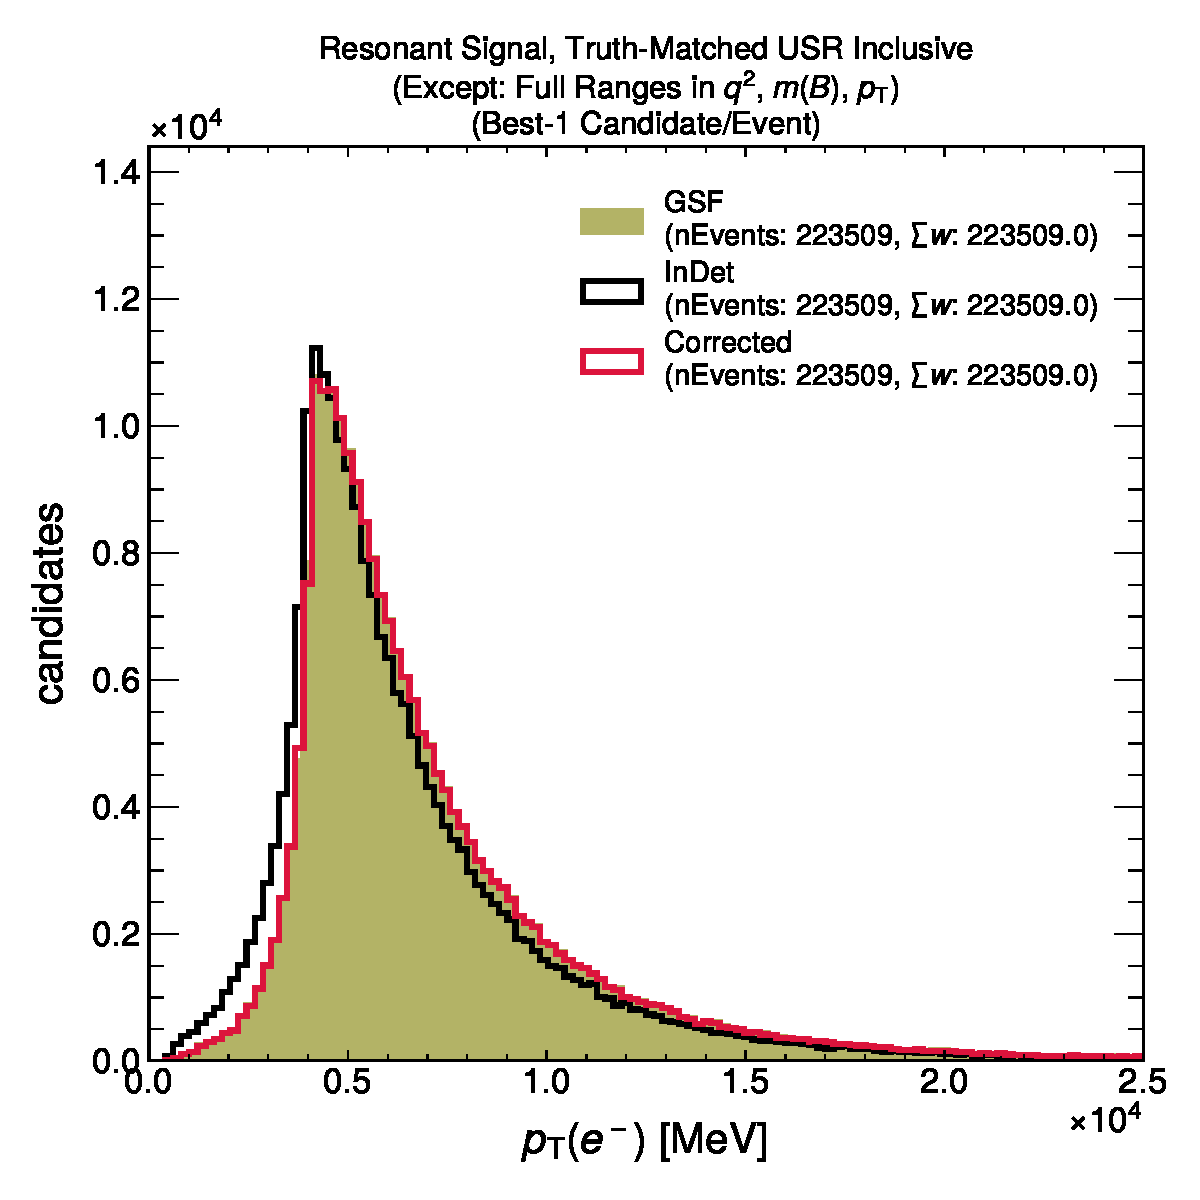
\includegraphics[width=\linewidth,page=1]{figures/FakesEstimation/InDetGSFCorrection.v2025.s1.Res.Thesis/closurePlots.individual.Corrected.Sample.ResSignal.Inclusive.USR.Except.FullQ2.FullBMassRegion.FullPt.TruthMatched.pdf}
        %\caption{$p_{\rm T}(e^-)$}
        \label{fig:sub3}
    \end{subfigure}
    \begin{subfigure}{0.45\textwidth}
        \centering
        \includegraphics[width=\linewidth,page=2]{figures/FakesEstimation/InDetGSFCorrection.v2025.s1.Res.Thesis/closurePlots.individual.Corrected.Sample.ResSignal.Inclusive.USR.Except.FullQ2.FullBMassRegion.FullPt.TruthMatched.pdf}
        %\caption{$p_{\rm T}(e^+)$}
        \label{fig:sub4}
    \end{subfigure}
    \vspace{0.1cm} % Adjust vertical spacing if needed
    \begin{subfigure}{0.45\textwidth}
        \centering
        \includegraphics[width=\linewidth,page=5]{figures/FakesEstimation/InDetGSFCorrection.v2025.s1.Res.Thesis/closurePlots.individual.Corrected.Sample.ResSignal.Inclusive.USR.Except.FullQ2.FullBMassRegion.FullPt.TruthMatched.pdf}
        %\caption{$m(e^+e^-)$} 
        \label{fig:sub2}
    \end{subfigure}
    \begin{subfigure}{0.45\textwidth}
        \centering
        \includegraphics[width=\linewidth,page=6]{figures/FakesEstimation/InDetGSFCorrection.v2025.s1.Res.Thesis/closurePlots.individual.Corrected.Sample.ResSignal.Inclusive.USR.Except.FullQ2.FullBMassRegion.FullPt.TruthMatched.pdf}
        %\caption{$m(B)$}
        \label{fig:sub1}
    \end{subfigure}
    \caption{Comparison of Kinematic Variables between GSF and ID Tracks for the Electron Channel}
    \label{fig:main-kinematic-correction}
\end{figure}
\end{comment}

\begin{figure}
    \centering
    % First row
    \begin{minipage}{0.45\textwidth}
        \centering
        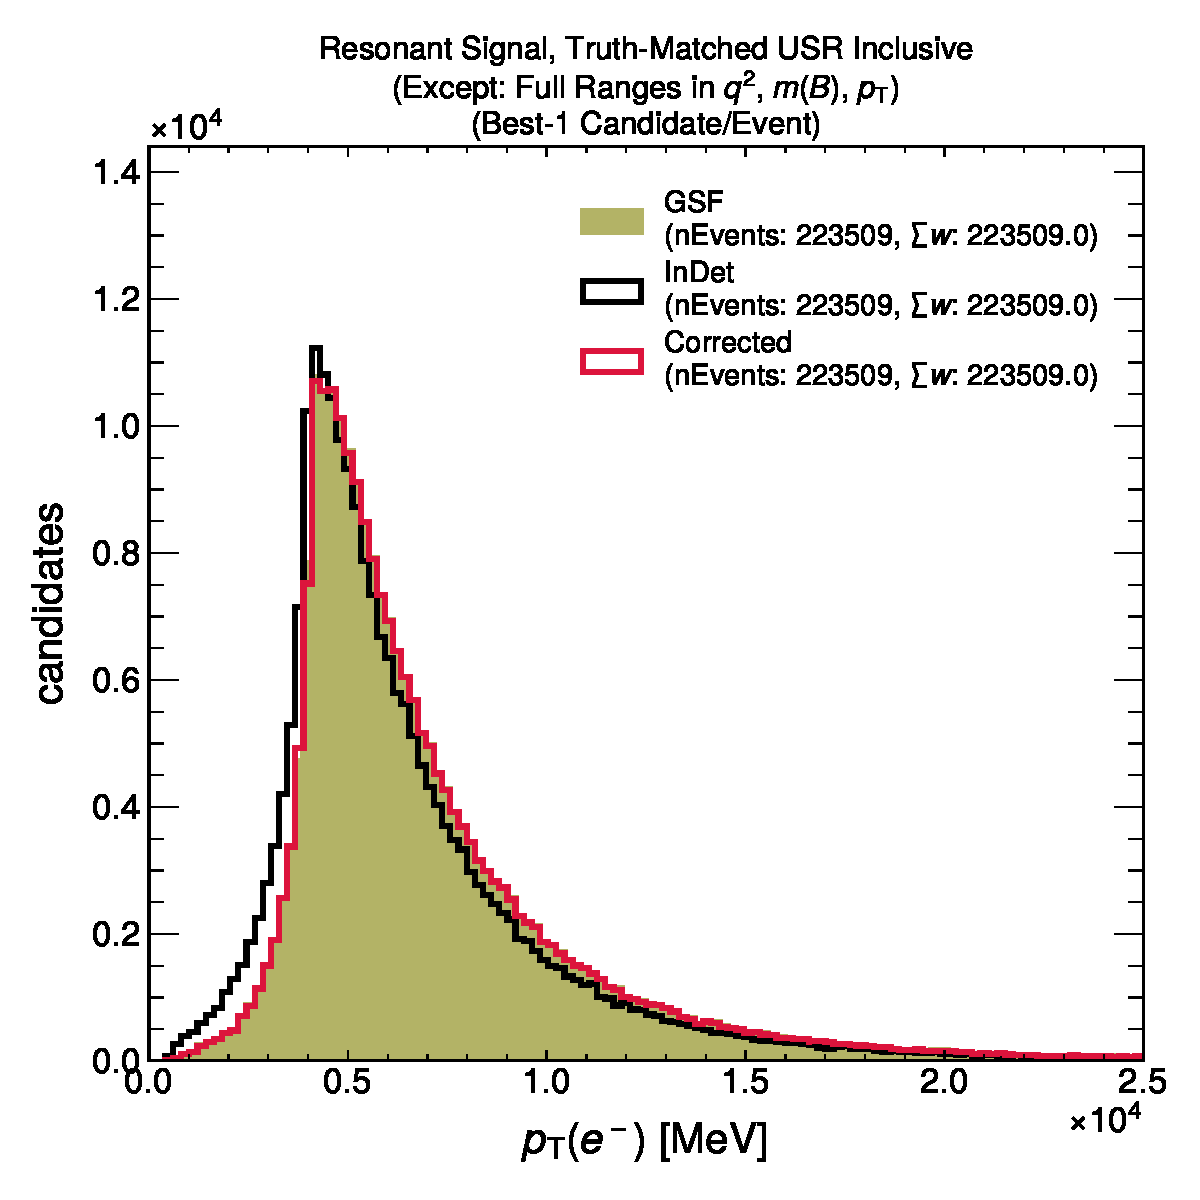
\includegraphics[width=\linewidth,page=1]{figures/FakesEstimation/InDetGSFCorrection.v2025.s1.Res.Thesis/closurePlots.individual.Corrected.Sample.ResSignal.Inclusive.USR.Except.FullQ2.FullBMassRegion.FullPt.TruthMatched.pdf}
        %\caption*{$p_{\rm T}(e^-)$}
        \label{fig:sub3}
    \end{minipage}
    \hfill
    \begin{minipage}{0.45\textwidth}
        \centering
        \includegraphics[width=\linewidth,page=2]{figures/FakesEstimation/InDetGSFCorrection.v2025.s1.Res.Thesis/closurePlots.individual.Corrected.Sample.ResSignal.Inclusive.USR.Except.FullQ2.FullBMassRegion.FullPt.TruthMatched.pdf}
        %\caption*{$p_{\rm T}(e^+)$}
        \label{fig:sub4}
    \end{minipage}
    \vspace{0.1cm} % Optional vertical space

    % Second row
    \begin{minipage}{0.45\textwidth}
        \centering
        \includegraphics[width=\linewidth,page=5]{figures/FakesEstimation/InDetGSFCorrection.v2025.s1.Res.Thesis/closurePlots.individual.Corrected.Sample.ResSignal.Inclusive.USR.Except.FullQ2.FullBMassRegion.FullPt.TruthMatched.pdf}
        %\caption*{$m(e^+e^-)$}
        \label{fig:sub2}
    \end{minipage}
    \hfill
    \begin{minipage}{0.45\textwidth}
        \centering
        \includegraphics[width=\linewidth,page=6]{figures/FakesEstimation/InDetGSFCorrection.v2025.s1.Res.Thesis/closurePlots.individual.Corrected.Sample.ResSignal.Inclusive.USR.Except.FullQ2.FullBMassRegion.FullPt.TruthMatched.pdf}
        %\caption*{$m(B)$}
        \label{fig:sub1}
    \end{minipage}

    \caption{Comparison of Kinematic Variables between GSF and ID Tracks for the Electron Channel}
    \label{fig:main-kinematic-correction}
\end{figure}


\subsubsection{Applying Trigger Weights}
\label{subsec:applying-trigger-weights}
To correct for the lack of trigger-level lepton identification criteria, we derive the probability that a given $B$-candidate will pass the trigger selection, given that it has passed the offline selection. %
Recall that we have already corrected for the lack of offline lepton identification criteria by applying the faking probabilities to the $B$-candidates. %
Thus, we assume that if a hadron passes the offline lepton identification criteria, then its conditional probability of passing the trigger-level lepton identification criteria can be approximated by the same probability for a real lepton. %
Thus, we can use the reference channel to derive the trigger weights. %
Currently, these weights are derived using the MC samples of the reference channels. %\DM{Say anything about data-driven?} %
These weights, intuitively, correspond to the probability that a given $B$-candidate will pass the trigger selection, given that it has passed the offline selection -- correspondingly, they are derived using the ratio of the number of events passing the trigger selection (and the offline lepton selection) to the number of events passing the offline selection. %
However, to take into account the effect of prescales that are not simulated in the MC samples, each of the events in the numerator of the ratio is weighted by the prescale weight. The details of how the prescale weights are derived are discussed in Appendix-\ref{sec:app-prw-math}. %
The trigger weights are parametrized in the $p_{\text{T}}, \eta$ of the two leptons and the $\Delta R$ between the two leptons. %
In order to avoid having to optimize binning in this $5{\text{D}}$ space, the parametrization is achieved using Gaussian Kernel Density Estimation (KDE). %
Thus, the trigger weights are given by:
\begin{align}
    w_{\text{trigger}}( p_{\text{T}}^+, p_{\text{T}}^-, \eta^+, \eta^-, \Delta R) &= \frac{\rho_{\text{trigger + prescale + offline}}(p_{\text{T}}^+, p_{\text{T}}, \eta^+, \eta^-, \Delta R)}{\rho_{\text{offline}}(p_{\text{T}}^+, p_{\text{T}}^-, \eta^+, \eta^-, \Delta R)}
\end{align}
where $\rho_{\text{trigger + prescale + offline}}$ is the density of the events passing the trigger selection (and the offline lepton selection) weighted by the prescale weight, and $\rho_{\text{offline}}$ is the density of the events passing the offline selection. %
The validation of the calculated trigger weights for the electron channel, using the reference channel of $B^0 \to K^\ast \ell^+ \ell^-$, is shown in \ref{fig:main-trigger-weights}. %
%\DM{Add the figure for the muon channel.}
\begin{figure}
    \centering
        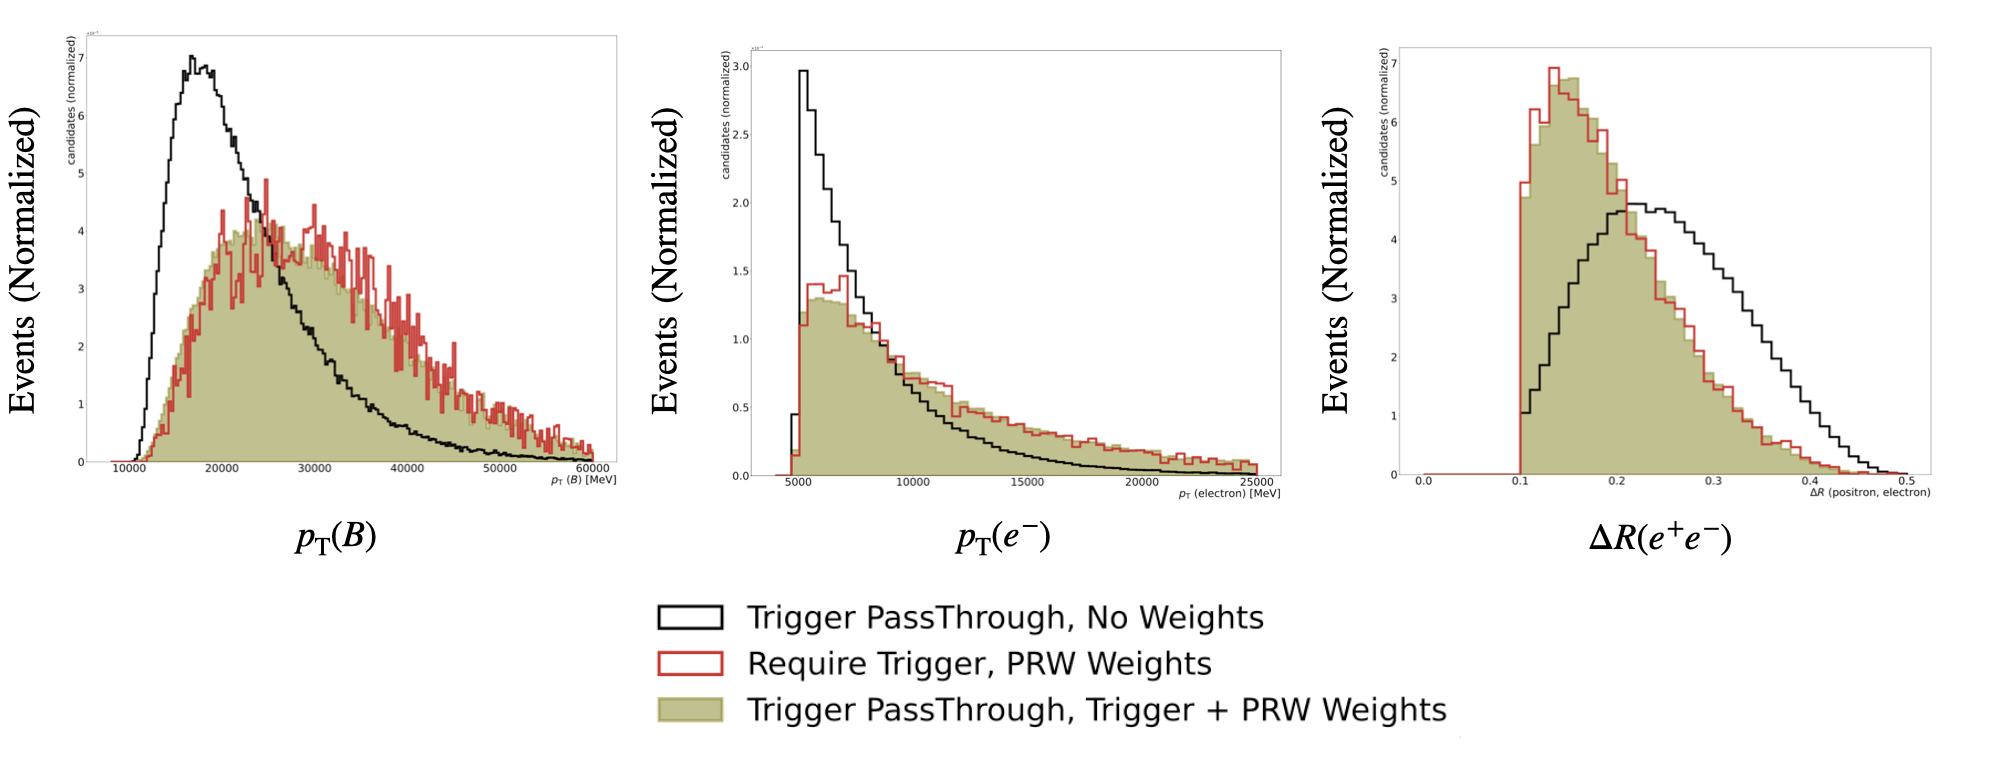
\includegraphics[width=\linewidth]{figures/FakesEstimation/trigger-weights-shapes.png}
        %\caption{$p_{\rm T}(e^-)$}
        \caption{Comparison of Kinematic Variables without Trigger Selection, with Trigger Selection, and with Trigger Weights for the Electron Channel}
        \label{fig:main-trigger-weights}
\end{figure}
